\chapter{ {Sailors} }

This is the first of two chapters that focus on socio-historical data about the sailors and their speech communities. This chapter specifically attempts to provide an overview on demographic data of English-speaking sailors of the early colonial Caribbean period by providing statistical (wherever possible) and qualitative data and in turn presenting the reasoning behind the capacity of this population to develop and sustain a distinct language variety. The chapter opens with a discussion of how sailors were recruited into maritime communities and subsequently presents sections that roughly correspond to census demographics: gender, age, health and mortality, family and marital status, social status, financial standing, place of origin, language abilities, literacy, and number of people residing in the ship community. 

\section{{General considerations}}\label{sec:3.1}

  Two problems characterize the misunderstanding about the people who worked and lived aboard sea-going vessels in the age of sail. The first problem arises from the uncertainty about the subjects discussed, while the second stems from the perpetuation of stereotypes in both popular culture and historical scholarship. The word ‘\isi{sailor}’ carries with it a presumption of lower-class manual labor, and this most probably derives from the original association of the word ‘\isi{sailor}’ with a \isi{seaman} whose job it was to manage the sails (\citealt{AdkinsAdkins2008}: xxvix). However, this definition is no longer what we mean when we use the word “\isi{sailor}”. In \isi{modern usage},  this term is generically used to refer to any employed \isi{seaman} and more specifically an experienced lower-class worker who is also explicitly an adult male, more appropriately correlating with the maritime rank “able \isi{seaman}”. This new definition, although more inclusive in scope than the original meaning, still does not include all the men, women, and children of different specializations, ranks, and experience who lived and worked aboard sea-going vessels. For example, the group denoted by the word does not typically include the maritime slave, the child apprentice, the captain’s servant, the marine, the ship’s doctor, the washerwoman, the carpenter, the landsman, and the admiral. Yet these people also lived at sea for significant periods if not the majority of their working lives. In contrast, the restricted group of lower-class experienced adult male workers who were free to enlist (i.e., the able \isi{seaman} that people often think about when they use the word “\isi{sailor}”) represents only one section of the population in a large vessel of the \isi{seventeenth century}. Thus, this chapter necessarily opens with a re-definition of the word to include all people, both male and female, young and old, experienced and novice, in all of the professions needed and preferred to navigate, defend, maintain, service, and populate the floating communities of large and small vessels in the early age of Atlantic \isi{colonial expansion}. 
–
  The perpetuation of the \isi{sailor} stereotype in both popular culture and historical scholarship is embodied by the term “Jack Tar”, a term notably used by officers to describe enlisted men since the 1600s that derived from the ubiquitous application of tar as a waterproofing agent in wooden ships coupled with the epithet “Jack” referring to the common man (for more extensive discussion see the book \textit{Jack Tar}, specifically pages, \citealt{AdkinsAdkins2008}: xxviii–xxvix). Perhaps, in part, because of this stereotype motivated by our restricted interpretation of the word “\isi{sailor}” we have typically failed to recognize the importance of real sea-going individuals in shaping our local and global histories. However, modern scholars such as Michael Jarvis are trying to recover the agency of individual sailors by recognizing that “[t]he decisions, innovations, adaptations, and self-organized enterprises of largely anonymous individuals shaped \isi{colonial expansion} and Atlantic history as much as imperial bureaucracies, state navies, chartered trading companies and metropolitan merchants” (\citealt{Jarvis2010}: 459). This chapter aims to promote the recognition of these “largely anonymous individuals” by recovering some of the demographic data that might help us understand who they were. 

Demographic data is in part recoverable, but the record-keeping of the community itself does not make this an easy task. Difficulties are compounded by the fact that these communities were transient, with high levels of illiteracy, and many individuals were often not considered relevant enough to remark upon in official records. Other individuals may have purposely concealed their identity, for example, the witness who explains that he changed his name because “he thought himselfe in ill companie” [ASSI 45/4/1/135] and the \isi{deponent} George Trivattin, who “After the pirating was committed [...] Changed his name to Edward Thomas” [HCA 1/14/154]. Others took false identities to evade or complicate the efforts of impressment officers and for this reason, many physical descriptions accompany the given name for newly enlisted men, for example, “Peter Fox abt 25 yeares old, of midle stature, slender body short fingers Reddish hair \& short, wearing at present a flaxen perriwig, smooth faite, a blark quick nimble eye” [HCA 1/101/411]. Transient sailors were also a difficult entity to determine, often navigating the undocumented frontiers between the mercantile and naval worlds \citep{Fusaro2015} or the logging, turtling, and salt-raking labor of the Atlantic commons (\citealt{Jarvis2010}). In short, in an effort to provide a comprehensive overview, the following sections on demography present data on sailors (redefined as all sea-going workers) that recognizes them as “highly complex \textit{individuals} with recoverable life stories, shoreside ties, ambitions, and more self-determination than is usually allotted them” (\citealt{Jarvis2010}: 465–466, author’s italics) yet also acknowledges the limitations and complexities of the data from which my conclusions derive. 

\section{{Recruitment}}\label{sec:3.2}

  Sailors were typically recruited rather than born into their communities and the various methods of recruitment for manning sea-going vessels affected the resulting demographics of the community. While most commanding and many commissioned and warrant officers were professionals who sought placement and promotion at sea, many of the petty officers, militia, and operational \isi{crew} would have been enlisted via methods involving some degree of coercion, manipulation, or outright force. Recruitment methods included voluntary enrollment, conscription, and the assignment of impressed, enslaved, or detained populations. Each of these methods is briefly discussed in the following paragraphs as a means to try and understand the common characteristics of the men they targeted. 

  The ideal method to cover the manning requirements of a vessel was by voluntary recruits, and this method was most successful for enlisting commissioned officers during the Anglo-Dutch wars of the \isi{seventeenth century}. Privileged second and third sons of the landed gentry not eligible to inherit titles often sought commissions and favor from family members to help them advance in the navy whilst at the same time fulfilling their desires to travel and build reputation (\citealt{Brown2011}: 53). In contrast, efforts to encourage volunteers for lower-ranked positions in the fleet was often less productive. The men needed for these positions would not enjoy the financial rewards and status associated with the ranks reserved for “gentlemen”,\footnote{“Gentleman” in this context refers to landed gentry and the adult males of wealthy families of the period without the intention of suggesting any personal respectability or strength of character.}  and their work was often hard and considered menial. Yet, popular broadsheet ballads commonly pandered to the working classes in order to motivate voluntary recruitment. Some songs glorified voyages, such as “The honour of Bristol”, (cited in \citealt{Palmer1986}: 24–26) that highlights the achievements of the ship \textit{Angel Gabriel}, a Bristol Privateer that allegedly fought with three Spanish ships in the late 1620s, killing 500 men and gaining glory and riches for the \isi{crew}. Other songs were much less factual, such as “Sailors for my Money” a self-conscious ditty that proposes to its readers, “Let’s sail into the Indies where the golden grass doth grow” (cited in \citealt{Palmer1986}: 29). Recruitment to the civilian fleets, including \isi{merchant} and \isi{pirate} vessels, offered more tangible incentives such as increased wages in times of high demand and shares in cargoes and captured goods; consequently, these fleets often enlisted more working-class volunteers than the navy. 

   Many working class sailors enlisted to escape poverty rather than to earn money. One volunteer states his reason, “not having any thing to Eat [...] I consented to goo” [HCA 1/98/44]. Another volunteer, hearing drums beat to announce recruitment, joined a group of would-be recruits that “desired the master to give them some victualls” [HCA 1/53/67]. Hugh Bicheno explains such motivation, in his \citeyear*{Bicheno2012} study of \textit{Elizabeth’s Sea Dogs}:

\begin{quotation}
Only abject misery can explain how anyone would volunteer to \isi{crew} the Queen’s ships. Although in theory sailors serving in the Royal Navy in 1588 were paid 7s.6d. per month, in practice they were paid late or not at all and had little prospect of spoil. The only certain payment was in kind: accommodation on board was better than sleeping in the streets or in dosshouses, and while the food and drink was usually rank and sometimes poisonous, the alternative might be starvation. (\citealt{Bicheno2012}: 182)\end{quotation}

The need for bed and board may explain why some volunteers came directly from other ships without staying in port, as attested to in one logbook entry, “I brought along with me about 40 men out of the York who Voluntary offer’d their services” [ADM 51/4322/4] and a passenger account of how “The \textit{English} [sailors] divided themselves, some aboard our ship, and some aboard the \textit{Turk}” [445f.1/513]. Likewise, acute financial need characterises the testimony of another volunteer who “[w]as forced to hide himselfe and goe to sea for Debt” [HCA 1/11/110]. Indeed, poverty was likely the motivating factor for the majority of lower-ranked men on ships in addition to those workers whose voices are not recognized in official documentation such as female servants, child workers and indentured peoples.

Impressing sailors to man naval fleets in times of war was a common strategy that goes back to medieval times in Britain. The impress service (colloquially known as the press gang) predominantly targeted experienced sailors with offers of advanced pay and was conceived as a heavy-handed push to motivate volunteer recruits. Logbook entries attest to the extensive nature of such practices, for example, sailing in March 1691, “the \textit{Mary} has presst all her men” [ADM 52/1/8] and The \textit{Albemarle} receives “a Pressing having In 60 men” [ADM 52/2/5] on December 29 1691. Even on a smaller scale, the practice was routine, as attested to in the logbook of the \textit{Antelope}, in a footnote that reads “to Day received 5 Prest men on board” [ADM 52/2/9] and an unnamed vessel that records how they “Came Downe here from London with 6 Prest men which ware putt onbord” [ADM 52/1/6]. Although the figure would have fluctuated in times of war and national need, the National Maritime Museum in London estimates that by 1790, some 16\% of sailors were forced by press gangs. This routine procedure was also used to recruit some of the higher-ranking warrant officers, for example, in his study of sickness and health at sea, Kevin Brown observes that “the majority of sea-surgeons and surgeons’ mates were pressed into service” (\citeyear{Brown2011}: 25) and the instructions for impressment in a letter from James City in Virginia, dated April 16 1700 specifies “Warrants for the impressing pylots, carpenters, or any other Workmen, as shall be necessary” [CO 5/1411/660].

The press was problematic however, and various documents attest to its inconsistent practices that coerced and exploited the poor. Although the press-gang was only meant to encourage seafaring volunteers, in practice they coerced landsmen, boys, vagrants, and convicts in addition to the forced conscription of seamen and port workers to complete crews of large naval warships in times of need. One letter dated March {1700} and signed by four representatives of the navy’s supply services describes how port trade is affected because “by the impressing of some of their men others are frighted from their duty” [SP 42/6]. Yet, local governments recognized that the dregs of their societies could be put to work in this way and invariably supported impressment officers if complaints made it to trial. This situation created serious problems of corruption, extortion and abuse in the impressment service and led to practices such as seizing men indiscriminately before extorting money to let them go with the threat of forcing them into conscription if the sum was not paid. Adkins and Adkins explain that poor men who were unable to pay the press gangs off were forcibly removed from their families, often without any recourse to bid farewell or explain the situation (see \citealt{AdkinsAdkins2008}: 43–58). In a contemporary diatribe of the practice, Lieutenant Haversham explains to Governor Vernon that the system is rife with corruption. He explains, “he that is prest may be represented by the press officer as coming voluntarily, especially when the press officer can find his own accts [rewards] in it, which I dont doubt but they may too often contrive to do” [SP 42/6]. As testimony to such coercion, the court records of a trial in 1722 describe a recruit who “had a trick put upon him there and was forced to make a sort of sale of himself to [an] officer for cleaning the Debt” [HCA 1/99/124]. As a result of such corrupt practices, the press-gangs were fiercely opposed and feared in equal measure and their appearance in port towns often led to rioting, murders and assaults committed on both sides. 

Repeated testimony in court records between 1620 and 1750 refers to the profusion and violence of impressment. One \isi{deponent} recalls how he was taken by press gangs at various times, and describes one of those experiences on land that occurred in 1660:

\begin{quotation}
I met four press-Masters, and I might have shunned them, but durst not; and when we met, they ask’d me, Whether I was a Master, or a Man; I denying to be a Master, they replied, you must go with us; not so, said I; then they took hold of me, two under my Arms, and another two under my Hams, and lifted me upon their Shoulders, and carry’d me about three hundred Yards [...] they heav’d me from their Shoulders, over the Wharf, cross the Boat-thaughts, which was about five Yards high; and had not Providence preserved me, they had killed, or else crippled me. [445f.1/26]\end{quotation}

The same \isi{deponent} relates a different experience with another press gang in 1662:

\begin{quotation}
No sooner we came to an Anchor, but a Press-Boat came on Board us [...] they ty’d a Rope about my Waste, and with a Tackle hoisted me; making a Noise, as if I had been some Monster; and lower’d me down upon the Main-Hatches. [445f.1/26–27]\end{quotation}

Other deponents talk about being beaten with sticks, tied with ropes, grabbed in the night, and duped into going aboard (see series HCA 1/99/11). Yet most poor sailors had no choice but to accept the situation as normal. It was just another hard fact of life that some crewmates, like \isi{sailor} David Creagh, were “kept in the Service by force and violence” [HCA 1/13/108]. 

  Although press gangs focused their efforts on the port towns of the British Isles, colonial ports were not exempt from impressment. The records of the Colonial Office include various letters from administrators complaining about impressment activity around the Caribbean and on the coastal plantations of colonial North America. For example, one letter complains “against pressing seamen in the [Virginia] plantatons” [CO 5/1411/558] and another demands that “Captains shall not for the future be permitted to press” and urges impressment officers to make sure that pressed men “be good sailors [...] and not to carry off any Inhabitants from the sd [said] plantation” [CO 5/1411/624]. Hence, the press was likely to enlist a cross-section of lower-class workers in and around Britain’s colonial holdings, regardless of profession, nationality, or native language who would disproportionately represent lower-class men of working age. These men were enlisted and kept in service by force, potentially subjected to confinement in the putrid darkness of a ship’s hold, guarded by soldiers, and denied shore-leave for fear of desertion. Yet, these were the “volunteers” of the Royal Navy in Britain during the sixteenth and \isi{seventeenth century}, and our recognition of their recruitment and experiences is an essential part of their demographic profile.  

Men could also be pressed into service directly from another vessel. This type of ship-to-ship impressment was abhorred by \isi{merchant} sailors with hopes of returning to their homes after an extended \isi{voyage} yet was common practice in naval recruitment and commonly known as “turning over” the \isi{crew}. Documentary evidence regularly refers to this practice, e.g., one \isi{sailor} writes “Yesterday My Self with the Rest of the \textit{Foresights} Company were turned over” [ADM 51/4170/2] and various logbook entries attest to large numbers of sailors coming from other vessels: “This morn Turned 20 men over Into the \textit{\isi{Essex} Prize}” [ADM 52/2/5]; “we have… this morn Sent 30 men on board the Dunkirk” [ADM 52/1/5]; “turned 50 men on board the Barwick” [ADM 52/2/3]; and more extensively, “Received on board out of the \textit{Arendall} men that she brought out of the Downes from severall shipps Viz the \textit{Colchester} 27 the \textit{Sohampton} 12 the \textit{English Begar} 11 the \textit{Woolwitch} 43 \& out of the \textit{Brittainia} ketch 50 \& out of the \textit{St. Michael} Smaek 29. In all 172” [ADM 52/2/5]. Even individual court testimonies reflect the movement of sailors in this manner, e.g., the description of one \isi{deponent} as “a Jersy Man forced out of the \textit{Success} Sloop in the West Indies” [HCA 1/99/89]. Colonial administrators were complicit in this practice, issuing warrants like the one dated January {1699} from Francis Nicholson, governor of Virginia and Maryland, who granted captain John Aldred permission “to impress one able \isi{seaman} out of any ship or vessel who hath fifteen \isi{seaman} or upwards” [CO 5/1411/665]. Indeed, turning over a \isi{crew} was such a successful practice for manning a vessel with experienced sailors that \isi{pirate} crews adopted the custom. George Bougee’s trial for piracy in October {1684} describes “30 and 40 men on board” captured from a taken vessel whose captain was on shore trading [HCA 1/12/1]. Yet, even in these non-negotiable transfers, captains attempted to coerce sailors to make declarations of compliance, e.g., in the September 9th trial records of Rhode Island and Providence Plantation 1725, one \isi{pirate} captain is accused of forcing potential recruits to eat candles and to run a gauntlet of sticks wielded by the \isi{crew} if they would not “volunteer” [HCA 1/99/5]. In the same trial, a witness testifies that the same “Capt Hunt… used him Barbarously threatening to cut of [off] one of his fingers for a ring he had on and Low beat out one of his Teeth \& threatened to Pistol him if he would not sign their articles” [HCA 1/99/7]. Contemporary courts acknowledged this type of coercion, as evidenced by some surviving documents attesting to coerced impressment, to be used as certificates in case of capture, e.g., “Evan Jones Acknowledging of his forcing the Freeland to goe his surgeon” [HCA 1/98/181] dated October 29 1699. Also, in the trail of March 28 1722, court officials decided to try every one of the 88 accused pirates individually under the recognition that “many of the Prisoners found on Board were new entred men and forced thro fear to act the Part they did” [HCA 1/99/3/16]. Thus, not only naval fleets, but also \isi{pirate} vessels were likely to have kept men for lengthy periods against their will and refused them any type of shore leave for fear of desertion. 

Sailors who were turned over were not the only non-consenting \isi{crew} members; \isi{indenture} and slavery were also common routes to sea service. Piracy trials often concluded with a term of service for men found guilty, e.g., the men tried on 28 March {1722} were punished each with a seven-year term of \isi{indenture} in the Royal African Company [HCA 1/99/174]. Boys and young men were also liable to be sold into \isi{indenture}, e.g., one young man’s description that “he was in a Storme at Sea in a Shipp belonging to Captain Thomas Shaft who was his Master, and with whom he hath lived 5 yeares, having bin bound to him for 7 yeares” [HCA 1/12/79]. Slaves were also used to complete crews, particularly in the privateer and \isi{pirate} fleets that were not subject to the same compliance with Britain's 1651 Navigation Acts that required a \isi{crew} to be at least three quarters British.\footnote{The {1651} Navigation Acts specifically applied to the returning voyages of East India Company Ships and restricted the employment of non-English sailors to a quarter of the \isi{crew}. However, their general aim to minimize foreign (and specifically Dutch) involvement in the colonial trade was legitimized by this legislation which was more widely applied that its originally specified scope.} The use of slaves in addition to indentured workers including vagrants, prisoners, and the destitute meant that non-consenting sailors were a core component of crews in the early \isi{colonial period} in addition to volunteers, conscripted men, and detained workers. 

\item \section{{Gender}}\label{sec:3.3}
\end{itemize}

  As previously acknowledged in the discussion of the Jack Tar stereotype, we tend to presume that all sailors were male and women’s presence on board was limited to the fleeting visits of prostitutes when stationed in port. Whilst it is no doubt true that the majority of sailors (i.e., all sea-going workers) were male, there was, nonetheless, a minority of women aboard. The presence of some of these women emerges in fleeting descriptions, such as the deposition of Anne Hoy in 1695, rather ambiguously described as “Liveing in Ship” [HCA 1/13/101].  It may have been that Anne Hoy was a personal servant, indeed, the most common role of these women who lived in the ships was in the guise of officers’ servants performing the work of food preparation, cleaning, and general maid’s duties, and potentially, even carrying gunpowder in times of conflict when enlisted men were operating the guns (as suggested in \citealt{Brown2011}: 95). As these workers were employed independently, they do not appear on the ship’s payroll and their work has consequently gone largely unrecognized. Yet, there is recoverable evidence of these women’s presence and agency aboard sea-going communities, e.g., Anne Foster, described as a maid servant suffering abuse from her employer [HCA 1/101/426], “Marramitta (my Negore) Cook” serving on board the \textit{Margarit} [HCA 1/98/100], and Rose Baldwin, Jane Alcocke, and Elizabeth Cammiothe who are described as servants aboard the \textit{Elizabeth and Mary}. Interestingly, in this case, the \isi{deponent} testifies that the three women “lay together in A Cabbin Standing neere the main mast between decks” [HCA 1/9/51] suggesting that there were allocated women’s quarters onboard. Yet, this piece of information only comes to light because two of the women are deposed to give evidence in the murder trial of a man who was chained to the main mast near their cabin. In the same trial, William Dunston testifies that the light he saw “might be any of the men Servants, Mayd Servants or any of the Seamen” [HCA 1/9/51], suggesting the notable presence of both male and female servants aboard the naval vessel. Similarly attesting to a notable female presence on board a 250-man vessel, one journal writer describes how “the cries of the women terrify’d those that were most inured to those tempests” [445f.1/516]. Such fragmentary evidence recognizes women’s work among sea-going communities despite the fact that they were unlikely to appear in any official ship’s muster or payroll. 

  Women worked as maids and servants yet they also worked as enlisted crewmen in the navy. Adkins and Adkins explain the long, if somewhat covert, tradition of women serving at sea as evidenced by “documented instances of young women passing themselves off as boys on both \isi{merchant} and naval ships” (\citealt{AdkinsAdkins2008}: 182). These include, for example, Hannah Snell’s publication of her experiences as a marine (published 1750) and Mary Lacy’s experiences as a carpenter’s servant and shipwright under the pseudonym William Chandler in the naval fleet, published in the compilation \textit{The Lady Tars} (\citealt{SnellEtAl2008}: iv). Popular ballads, stories and songs also testify to the tradition of female \isi{crew}, exemplified by titles such as “Susan’s Adventures in a Man-of-War”, “The “Female Tar”, and “The Female Cabin Boy” (cited in \citealt{AdkinsAdkins2008}: 181–182). In short, in spite of their own efforts to conceal their presence, recoverable evidence of their agency attests to their service in the navy. 

Women were also active in \isi{pirate} communities as evidenced in court records of trials. Aside from the more famous examples of pirates like Anne Bonny and Mary Read whose agency was recognized during their lifetimes (see \citealt{Rediker2004}: 103–126), there were potentially many women who collaborated in piratical activity and served aboard \isi{pirate} vessels, yet for whom we have either no record, or only fragmentary and circumstantial evidence. For instance, the witness testimony of a \isi{prisoner} on a \isi{pirate ship} explains how he and his men were “put down into the Cabbin and the Scuttle or hatch shut, and Mary Critchett sat down on it to keep the Deponent from opening it” [HCA 1/99 \isi{Williamsburg}, Aug 14 1729]. Another document dated September 28 1638 includes witness testimony of Jane Handall and Margarett Pope, both charged with piracy. In her testimony, Pope accuses “Jane Handall being Damamed if she Did not Helpp her Husband about the tyme aforesaid” [HCA 1/101/252] suggesting that the husband and wife team worked in collaboration. Yet, despite these few documented references to the agency of women on board \isi{pirate} ships, admiralty officials of the era rarely noted the presence or contributions of women on board any English \isi{pirate}, naval, or \isi{merchant} vessel. However, as Murphy explains in his \citeyear*{Murphy2015} conference paper on women in the navy, the English civil war in the \isi{seventeenth century} forced many women to seek refuge on ships and these women likely worked in whatever capacity would gain them a berth on the ship. In short, we must accept that the demography of sailors’ communities during this time necessarily included a minority of female \isi{crew} and service providers beyond the caricature of the port prostitute. 


\section{{Age}}\label{sec:3.4}

  Determining the average ages of a population for whom documentary evidence is fragmentary and incomplete poses significant difficulties, yet, generally, we can assert that sailors were young. Peter Earle, a scholar who has done extensive work on age demographics of English sailors of the period under study, determines that the majority of sailors went to sea between the ages of 12 and 16 (see \figref{fig:key:3.1}  adapted from \citealt{Earle1993}: 85). Additionally, the likelihood of children serving on vessels was increased by the practice of sending vagrant children to populate the English settlements in Virginia (shipments sent in 1619, 1620, and 1622) and also the custom of spiriting (i.e., kidnapping) children for work in the Americas, resulting in large numbers of children in the working Atlantic [\isi{Merseyside} Maritime Museum, Information sheet 10: Child Emigration]. Testimonies of teenage sailors abound in court documentation, for example Stephen Bakes who went to sea as carpenter’s mate at age 17 [HCA 1/13/97] and Thomas Francois de Fouret who served as a clerk in a man of war at age 16 [HCA 1/13/96]. Yet, even in their teen years, some sailors were considered too young for certain types of work; one sailor testified at the age of 17 that, despite his rank as yeoman of the stores, “being underAge he was never allowed to go on Board of Prizes” [HCA 1/99/148]. Other types of work were specifically designed for younger workers. Among officers, entry level was at 11 years for a volunteer first class or 13 years if not the son of a naval officer (\citealt{AdkinsAdkins2008}: 64), yet rules were broken to permit younger recruits to acquire the 6 years’ sea-service expected before making midshipmen level in the army. Among the lower-ranking sailors, the position of “Boy, Third Class” was created specifically for those under the age of 15, many of whom appear in the court records, for example, William Muller, servant to an officer at age 12 [HCA 1/52/176] and Peter Killing, a boatswain's boy at age 13 [HCA 1/48/102]. Among the list of 98 pirates captured in one court record, three are described as “boys” and one specifically listed as “10 ys old” [CO 5/1411/826–27] suggesting that very young sailors were potentially on board. The youngest recruit I found evidence of in the records was Francis Longley of \isi{Jamaica} deposed at “about 12 years of age” who explains that he set out on a trading \isi{voyage} about four and a half years ago, making him eight years old at most when he joined the \isi{crew} [HCA 1/52/104]. Although Earle notes that such very young boys were by no means typical (\citealt{Earle1998}: 20) there are repeated references to schoolteachers aboard naval vessels, for whom instructions were provided that indicate the young ages of their pupils: “When the hatchways are open, the youngsters should always be cautioned against playing inadvertently near them; and care should be taken at the same time to tighten a rope around them, to prevent accidents, if possible” (in a manual published 1801, cited in \citealt{AdkinsAdkins2008}: 21). It is a sad fact that some of these boys may have been recruited for sexual exploitation, as discussed in \citegen{Burg2007} \textit{Boys at Sea} and in \citegen{Fury2015} discussion of the abuses that happened on the voyages of the East India Company. In sum, although the great majority of sailors were likely to have gone to sea between 12 and 16 (comparable to occupations on land), younger recruits were also employed, provided for, and used to service the needs of the \isi{crew}.


\begin{figure}

\caption{\label{fig:key:3.1}Age at which deposed sailors said they went to sea, adapted from the data presented in \citealt{Earle1998}: 85 Table 6, source: PRO, HCA 13/75–86}
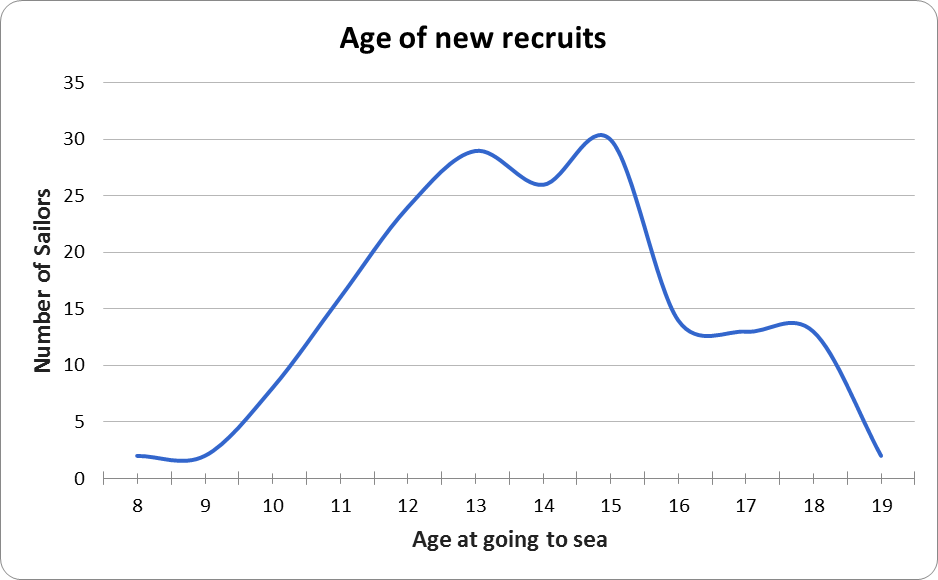
\includegraphics[width=\textwidth]{figures/delgado-img2.png}
\end{figure}

The upper age of sailors, as suggested by the few academics who have worked on this subject and corroborated by depositions in court documentation of the 1620–1750 period, is around fifty years old. At the age of fifty, and particularly if he had been at sea most of his working life, a \isi{sailor} would be considered old.  In his journal, physician Gilbert Blane notes:

\begin{quotation}
[seamen] are generally short lived, and have their constitutions worn out ten years before the rest of the laborious part of mankind [manual workers]. A \isi{seaman} at the age of forty-five… would be taken by his looks to be fifty-five, or even at the borders of sixty. (cited in \citealt{AdkinsAdkins2008}: 88) \end{quotation}

Archival records contain evidence of such professional seamen serving into their forties, e.g., the witness John Morphey, deposed at 46 years of age, who testifies that, since the age of ten, he “was bred up to the sea and hath ever since lived as a \isi{seaman}” [HCA 1/53/9]. Yet, if sailors could avoid the natural hazards of a life at sea, then it was entirely possible for them to serve until a more advanced age. For example, the HCA 1/53 batch of depositions dated 1694–1710 include one \isi{mariner} “George Burgis of Boston in New England \isi{mariner} aged about 67 yeares” [HCA 1/53/66] and another aged seventy [HCA 1/53/22]. The oldest \isi{deponent} in the HCA 1/52 batch of court records dated 1683–1694 was seventy years of age, and the oldest \isi{deponent} in the HCA 1/51 batch of court records dated 1674–1683 was a Waterman named Thomas Lowell, aged eighty-six [HCA 1/52/104]. Thus, although the average upper age of working sailors might be around forty-five, some survived to serve into more advanced years. It is also worth noting that there was an increase in the recruitment of very old and very young men on the \isi{merchant} fleets in the wartime periods of heavy impressment (mostly between 1689–1713) because these individuals were excluded from the press and thus protected from being poached by naval vessels seeking men to turn over. For example, sixteen-year-old Edward Lindsfeild deposed in a court case of 1692 that they sailed “with two, three or four boyes, feareing to carry men last they should be imprest” and Edward Round, age 76, gave evidence in the same case (cited in \citealt{Earle1998}: 200). 

 The average age of ships’ crews is just over thirty-one, based on the of ages of sailors for whom ages are recorded in 1,101 depositions collected by the High Court of the Admiralty between 1601 and 1710 (see \tabref{tab:key:3.1}). Yet this number may be inflated by the fact that men called to give evidence in court were often deposed due to their long experience at sea.\footnote{This explanation accompanies Earle’s data on median ages of sailors, officers and captains based on depositions in the collection HCA 13/75–86, a collection also included in my data (\citealt{Earle1993}: 86–87).} Furthermore, many of the court records derive from trials of piracy, in which we might anticipate that many \isi{crew} members were recruited directly from another vessel and hence spent time at sea already. If such a bias affects the data, then an adjusted average might be slightly lower, potentially in the late twenties.

The age composition of the \isi{crew} would naturally reflect the age demographics of different ranks. For example, the average age of captains and officers was between thirty-five and forty-four \citep[86]{Earle1998}; the average age of shipmasters was between twenty-five and thirty \citep[38–39]{Walsh1994}; and the average age of common sailors was between twenty-five to twenty-nine \citep[86]{Earle1998} although this last category of “\isi{sailor}” defined by Earle as “mariners, foremastmen, cooks, stewards, boys, apprentices, etc”. (\citeyear{Earle1998}: 86) was likely to have the most variation as it included the youngest apprentice to the oldest cook, a role often given to a disabled or aging \isi{seaman} and equitable to semi-retirement on the ship. In short, evidence suggests that the lowest ranks were in their late twenties, middle ranking officers might be in their early thirties and commanding officers might be around forty years old; however, it is important to remember that all of these data only reflect enlisted and documented sailors, typically of the navy, and fail to acknowledge the servants and slaves that were also likely to have composed the crews of naval, \isi{merchant}, and independent vessels. 

\begin{table}
\caption{\label{tab:key:3.1} The average age of seventeenth century ships’ crews based on ages of witnesses deposed in court cases, sourced the records of the High Court of the Admiralty at The National Archives, Kew}

\begin{tabularx}{\textwidth}{>{\raggedleft}p{20mm} >{\raggedleft}p{16mm}>{\raggedleft}p{16mm}>{\raggedleft}p{18mm} Q@{}}
\lsptoprule

 \textbf{Average age \mbox{of deponents}} &  \textbf{Youngest deponent} &  \textbf{Oldest deponent} &  \textbf{Number of deponents} &  \textbf{\mbox{Nat. Arch. Collection}}\newline \textbf{(date range)}\\
 \midrule
 37.4 &  15 &  60 &  68  &  HCA 1/49~(1622–1633)\\
 34.8 &  13 &  58 &  161 &  HCA 1/48~(1614–1620)\\
 33.1 &  12 &  72 &  168 &  HCA 1/47~(1609–1612)\\
 31.3 &  12 &  55 &  187 &  HCA 1/46~(1601–1607)\\
 31.1 &  12 &  70 &  177 &  HCA 1/53~(1694–1710)\\
 30.7 &  13 &  64 &  86  &  HCA 1/50~(1634–1653)\\
 29.6 &  19 &  40 &  22  &  HCA 1/9~~(1666–1674)\\
 29.0 &  10 &  58 &  171 &  HCA 1/52~(1683–1694)\\
 27.6 &  12 &  59 &  40  &  HCA 1/14~(1696–1700)\\
 26.2 &  18 &  50 &  21  &  HCA 1/13~(1692–1696)\\
 \midrule
 \textbf{Avg.: 31.0} &  \textbf{Avg.: 13.6} &  \textbf{Avg.: 58.6} &  \textbf{Total: 1,101} & \textbf{Total: 10 collections (1601–1710)}\\
\lspbottomrule
\end{tabularx}
\end{table}
\section{{Health and mortality}  }\label{sec:3.5}

Although generally, standards of personal health and hygiene were lower in the \isi{seventeenth century} than we might expect today, maintaining personal hygiene aboard ship was particularly challenging in cramped and overcrowded conditions with restricted access to clean water. Despite this, the \isi{common sailor}’s lack of personal hygiene was often considered part of their low character; a sentiment echoed in modern scholarship, for example in Bicheno’s observation that Queen Elizabeth’s “Royal Navy was largely manned by the dregs of the population, pressed into service along with their dirt, parasites and diseases” (\citeyear*{Bicheno2012}: 262). In response to health concerns, the Admiralty put measures in place to help sailors stay healthy in a challenging environment, such as the procedure of issuing \isi{seaman}’s clothes that came into effect in 1623 in an attempt to prevent the spread of disease (\citealt{Brown2011}: 31). However, measures taken to address the health of common seamen were often underfunded and unsustainable, such as the commission appointed for the care of sick seamen, established in 1664 and discontinued in 1674 (\citealt{Lincoln2015}: 145).

  Personal hygiene might have been improved, but it was the limited access to a balanced and nutritious diet that caused more sickness and disease than any other factor at sea. Contemporary sea-songs such as “The Sailor’s Complaint” reflected the impact of a poor diet and Palmer’s collection of songs explains that “food was the subject of perennial complaint by \isi{seaman}. Rotten meat, sour beer, smelly water, cheese hard as wood, biscuits full of weevils: the litany was long, and usually justified” (\citealt{Palmer1986}: 72). Ships’ logs and personal letters corroborate this situation, ranging from the mild complaint of “some bread decay'd” [ADM 106/300/16] to the more commonly recorded practice of condemning stores of food because of their poor condition, e.g., the description of bread, butter and cheese, “all rotten and stinking not fitt for men to eate” [ADM 52/2/5] and “two buts of beer Stinking…[and] 3 bushell of pease and on gall ould musty and roton” [ADM 52/2/3]. The end result of such provisioning meant that sailors often became, at best, “very Weak for want of Sustenance" [HCA 1/99] or, at worst, suffered from food-related disease and death. This may, indeed, explain the profusion of references to long, unspecified illness in contemporary accounts, for example the \isi{sailor} who “with the sickness [...] Confined so 3 or 4 Months” [HCA 1/99/159] and another who “had been sick Seven or eight Months” [HCA 1/99/127]. Other accounts make specific reference to scurvy which became a pandemic among maritime communities when vessels began to make longer voyages and increase time spent at sea without access to fresh food. In such contexts of food scarcity, it was not unusual for the \isi{crew} to resort to extreme measures. The curate passenger of a \isi{voyage} across the Atlantic in 1666 describes the piteous situation that the \isi{crew} found themselves in after seven months at sea, “after consuming all their provisions, to eat the cats, dogs, and rats that were in the ship… only five remained of four hundred men” [445f.1/486]. Yet, during a time of widespread starvation in the colonies and poverty among rural poor in Britain, the poor state of sailors’ health in relation to food security was nothing exceptional. 

  Sailors’ mortality rates are perhaps best introduced with the observation of a passenger on a \isi{transatlantic} \isi{voyage} in the \isi{late seventeenth century} who comments, “tis a sort of miracle we should live amidst so many hardships” [445f.1/486] or the observation of one anonymous sixteenth-century \isi{sailor}:

\begin{quotation}
mariners are but slaves to the rest, to moil and to toil day and night [...] and not suffered to sleep or harbour themselves under the decks. For in fair or foul weather, in storms, sun, or rain, they must pass void of cover or succour. (cited in \citealt{Lavery2009}: 28) \end{quotation}

Personal communications attest to the routine presence of death aboard ship, for example one letter observing that “we make nothing of burying 3 men in a day” [ADM 52/1/8] and another author’s stoic comment “One Plamber is dead and we want two more” [T 70/1/10]. Logbooks give similarly routine accounts of death, for example, “by Accident one of our men was Drowned” [ADM 51/3797/1], “faire weather and Little wind. dyed some of our Saylors. The wind varyable from the SS Et” [ADM 52/3/7] and “got to St. Marys; where the men did mostly die” [HCA 1/98/262]. Many records refer to the death of unnamed sailors for unnamed reasons and so we can only assume that such high mortality was common. Bicheno supports this assumption, explaining that \isi{sixteenth century} military victories were “marred by the death of hundreds of sailors from disease and want” (\citealt{Bicheno2012}: 259). Peter Earle provides a potential baseline for mortality statistics among maritime workers, claiming that due to accident, disease and violence, “around five percent of Bristol’s sailors were lost every year” (\citealt{Earle1998}: 87). In comparison, Jarvis’ work on smaller colonial communities with maritime economies suggests that “between one-third and one-half of all Bermudian men who went to sea died [at sea]” (\citealt{Jarvis2010}: 261). Hence, based on the contemporary accounts of routine death and the concurrent opinions of scholars working on different maritime populations, high mortality rates characterized maritime communities. 

The high mortality rates among sailors may have a link with issues of food security and personal hygiene, but they also likely derive from military conflict, the hardships of the work, environmental factors, and personal violence. Heavy casualties and loss of life among lower classes characterizes the type of military conflict of the era, and this was no different in the maritime communities that formed the heart of Britain’s fighting forces. Rival nations clamoring to claim the New World perpetuated various human rights abuses on all sides, e.g., “the killing of an English ship captain in Havana, merely for having requested water” [deposition of Henry Wasey, CO 1/23 cited in \citealt{Hatfield2016}: 12). The hardships of work on a wooden sailing vessel also potentially increased mortality rates, particularly when, as illustrated by this logbook entry, “the ship was very old and leaky” [HCA 1/52/76]. Examples of labour-related deaths include “a man putting the main sheates out [...] drowned” [ADM 52/2/1] and “six men died at their pumps with hard work” (cited in \citealt{AdkinsAdkins2008}: 117). Yet the ship may have been the safest place to be considering the range of environmental hazards that sailors also had to contend with including storms, yellow fever, malaria, smallpox, heat stroke and biting insects. The weather was also a major factor affecting mortality, e.g., “There hapned a very great storme [...] Ships bound from Barbadoes for England were all lost none of the said ships nor any of the Marrinrs on board them being ever heare off since to come alive to any place” [HCA 1/14/16]. Also, \citegen{Gage1648} survey of the West Indies describes some of its environmental hazards: “the abundance of gnats is such, which maketh him to take no joy in his voiage, and the heat in some places so intolerable, that many doe die” (p.186). In other accounts, horrific pandemics are described dispassionately e.g., “the small pox still Amonst us” [T/70/1216/13]. Even attempts at leisure were replete with danger in the \isi{sailor}’s everyday life, for example one description of how “the Mariners fell to washing themselves and to swimming” until one was attacked by a shark which “made them suddenly leave off that sport” (\citealt{Gage1648}: 20). Lastly, ubiquitous violence aboard sailing vessels, either in the guise of discipline, piratical activity, or personal grievance, increased the mortality rates of sailors as evidenced in “The Petition of a woman who prosecuted a master of a ship, for beating her son to Death” [HCA 1/101/225], and the \isi{pirate} attack in which “his throat was cut and belly burst so that his bowells came out” [HCA 1/52/137]. High mortality was therefore not only an occupational hazard, but also a characteristic of sailors’ communities that was exacerbated by cultural and environmental dangers. 

Seamen lived in conditions that were physically very close and this promoted the spread of disease. The lowest ranking men in naval warships were assigned 14 inches width to hang a hammock, although the spaces were alternated by watch and so this effectively doubled to 28 inches if the adjacent space was free (\citealt{AdkinsAdkins2008}: 188–189). In such confined spaces, illness often spread by contact, e.g., in the \isi{seventeenth century} large-scale outbreaks and epidemics affected naval fleets, such as the typhus outbreaks of 1625 and 1627 (\citealt{Brown2011}: 31). The idea of sick ships’ crews was no new concept however, throughout the middle ages epidemics of the Black Death that were associated with ships and trading ports of the Mediterranean (\citealt{Brown2011}: 2). In fact, the spread of infectious diseases could be interpreted as a somewhat pejorative metaphor of \isi{language contact} and feature transmission among port communities as in both respects the physical proximity of mariners are key to the process of transmission. To explain further, the bubonic plague spread by the bite of the \textit{Pullex irritans} flea which had been infected by the black rat \textit{Yersinia pestis} (more widely known as “the ship rat”) that infested \isi{merchant} ships and often came ashore even when the mariners did not. Proximity was critical to the transmission in much the same way that \isi{language contact} is crucial to feature transmission. The rat did not have to be in close or prolonged proximity to port workers in order for the flea to have an effect; and it is possible that language features could similarly have jumped ship even when mariners remained on-board. In another example, Yellow Fever, itself named for the yellow quarantine flag that would have been flown on an infected ship, after being first reported outside Africa in \isi{Barbados} in the mid \isi{seventeenth century} quickly spread around the trading ports of the Caribbean, to New York in 1668, Philadelphia and Charleston in 1690, and Boston in 1691 in addition to a southward spread to the trading ports of Colombia, Ecuador, and Peru (\citealt{Brown2011}: 116). Just as infectious diseases proliferated among ships crews and spread outward to coastal communities and inland waterways before affecting land-locked areas, it is entirely possible that language features were making the same journey. 

\section{{Family and marital status}}\label{sec:3.6}

  Sailors were not always the single and free young men that stereotypes perpetuate; they had strong familial bonds and many worked hard to provide for their wives and children. Jarvis notes that, particularly in Bermuda, kinship defined the ownership and operation of the short-distance trade that made up the majority of the island’s maritime activity (\citeyear*{Jarvis2010}: 121). Evidence of strong family ties, mostly retrieved through personal letters, suggests the value and influence of kinship among sailors, e.g., a letter from Evan Jones to his father that states “I believe you shall not hear from me again this 5 years [...] but my Duty to you and Love to brothers and sisters and service to my Unkle” [HCA 1/98/183] and another that refers to the writer’s “dutey to my father and mother and my Love to my sisters and brothers” [HCA 1/98/182]. The words “duty” and “service” in such personal letters suggests not only a respectful tone in comparison to the word “love” used when referring to siblings, but also potentially refers to the older generation’s investment in the \isi{voyage}. Such an interpretation is supported by Walsh’s observation that sailors of the English colonies were often bred into service at sea and supported by a father or an uncle until they married in their mid-twenties (\citeyear*{Walsh1994}: 28–34). He further explains that, as a result, contact with and duty to the parental generation was paramount for many sailors, so much so that it was sometimes explicitly stated in ships accounts that wages should be paid to the \isi{sailor}’s father or widowed mother (\citealt{Walsh1994}: 34). In this context, it is perhaps not surprising that, among miscellaneous documents of the Admiralty between 1620 and 1750, various letters addressed to fathers express duty and service alongside more traditional loving sentiments intended for sisters, brothers, cousins, nieces and nephews.  

  Sailors served at sea alongside family members. \citet{Jarvis2010} gives various accounts of small Bermuda sloops that were manned by kinship groups, and this practice also extended to larger vessels. Evidence of what seems to be fathers and sons serving together shows up in ships’ muster documents, for example “Robert Hartley (1st) and Robert Hartley (2nd)” [HCA 1/99/3/4–5] and in another vessel, “William Williamson” (1st) and “William Williamson” (2nd) [HCA 1/99/3/11–13]. Some court documentation also suggests the commonality of fathers and sons serving together, such as the decision of the court in one \isi{Williamsburg} trial on 14 August {1729} when “they agreed to discharge the \isi{deponent} and his servant, who had all along passed for his son” [HCA 1/99].  Brothers also served alongside each other, such as James and Henry Adams who testify in a \isi{piracy trial} 23 October {1699} [HCA 1/14/166] and Valentine Roderigo who testifies in a court of \isi{Bahama} Island 1722 that he was travelling to join his brother in Havana [HCA 1/99]. Not only immediate kin, but also the wives of mariners joined their husbands at sea. Brown explains, that many wives of common sailors were “smuggled aboard without the knowledge of the officers, [in addition to] [...] the wives of warrant officers, such as the gunner, carpenter, and purser” (\citealt{Brown2011}: 95). The fact that the East India company forbade their officers from taking their wives to sea in the early voyages of the \isi{seventeenth century} attests to the commonality of the practice as well (\citealt{Fury2015}: 16). Court documentation also records the presence of wives at sea, for example: Martha Farley who accompanied her husband aboard a \isi{pirate ship} and stands trial alongside him [HCA 1/99/8]; Elizabeth Trengove, described as a passenger of the \textit{Onflow} accompanying her husband, Captain Trengove [HCA 1/99/79]; and the unnamed woman mentioned in the description of how one \isi{sailor} “went down in a canoa with his wife” [HCA 1/99/7]. Additionally, the repeated use of the title “sea wife” in court appears to refer to women who accompanied their husbands to sea, for example: Anne Seayford [HCA 1/47/76], Alice Reeve and Anne Fladds [HCA 1/47/312], Elizabeth Leech [HCA 1/48/26], Ellen Rippingham [HCA 1/48/27], Margarett Weedes [HCA 1/48/29], and Dorothie Cooper [HCA 1/48/240], who are all referred to as “sea wife” in court records. In sum, sailors may have been accompanied to sea by a variety of family members, particularly in small sailing craft owned and operated by kinship groups, but even in large ships, sailors may have worked alongside fathers, uncles, brothers and wives. 

  Even when unaccompanied by their wives at sea, male sailors of age were likely to be married. Miscellaneous documentation of the Admiralty collection includes numerous letters that sailors wrote home to their wives expressing loving sentiments, such as this example sent in 1607 that not only elicits communication in return, but also expresses earnest desire to be reunited:

\begin{quotation}
My dere Love this is to satisfie you that I am on bord in gottenberg and came safe over [...] I am in very good health [...] and am thies day going with a small vessel for kopon hagen and hoping to get thither with five days and as soon as I kan get thether schall I write to my der Loving wife that my dearest may know how to send Letters to mee…[I am] thinking pon by dearest Love how god shi as to mee, and is me so alloen amongst a Compani of bad pipoll and when I doe soe Consider of it then it Cutts mee to the very hart [...] I am not at rest [...] for I can get a llatter from my dere Love [signed] your derest Loving husband. [HCA 1/101/527]\end{quotation}

This type of letter is often accompanied in the archival records with a reply from the \isi{sailor}’s wife with similar sentiments, for example “Deare And Loving husband [...] with Dayly wishes for your Company” [HCA 1/98/116]; “Deare Jacob [to let you know] How it is with mee and your Children” [HCA 1/98/118]; and “[I] shall ever prey for your safe retorne \& am your ever dutyfull \& loving wife” [HCA 1/98/51–52]. Despite the stereotype of the profligate wanderer, it is clear that many sailors advocated for marriage, as expressed in the advice to a friend drafted on the back page of the \textit{Pideaux}’s logbook “when you gett home that I would advise you to Mary with your old sweethart Elizabeth Raglis and not to lust after other women” [HCA 1/99/50]. Another married \isi{sailor} describes a friend: “hi wants a vry god wife but hi is afraid [...] of thorty yers of age” [HCA 1/101/528] before he requests his own wife to find his friend a suitable match. Although the majority of letters that are recoverable reflect the sentiments of literate midshipmen and commanding officers, there is no reason to assume that less literate sailors on board did not also marry and cherish women in their lives. Indeed, evidence of lower-ranking married sailors is recoverable from Admiralty records, e.g., depositions such as Lewis Innes who refers to his wife [HCA 1/99] another anonymous \isi{sailor} who testifies that “he hath lived at Dunkirk abt one year \& a halfe and hath a wife \& family living there” [HCA 1/52/100] and the simple testimony of another that “he had a family” [HCA 1/99/85]. Other documentation also corroborates the marital status of common sailors, for example, the letter that John Morris dictated on his deathbed after being savagely beaten by the ship’s mate to his “Ever Loufing wief” entrusting her with the information and witness testimony to challenge the chief mate after his death and signed with the shaky initials of the barely literate [HCA 1/52/51]. Wills and inventories in Bermuda also list items that sailors gave to their wives \citep[214]{Jarvis2010} perhaps explaining the presence of a “a pair of women’s shoes” among the contents of a \isi{sailor}’s chest itemized in court [HCA 1/99/8]. Additionally, Brown notes, it was common practice for a low-ranking \isi{sailor} to have his clothes and other personal possessions returned to his wife in the event of death at sea (\citealt{Brown2011}: 26). Hence, although fragmentary and incomplete, there is sufficient evidence to show that not only literate classes of sailors married but also that many lower-ranking workers on the ship were married men too. 

The wives of these sailors may have formed a critical support network in port communities. Some wives managed a variety of caregiving responsibilities. For example, Admiralty records of a \isi{sailor}’s trial dated 17 December {1687} describe “a Woman coming into Court, and declaring that she had kept his Child and been at 20l. charge” [HCA 1/12/111]. Additionally, among the miscellaneous documents about the ship’s business, Thomas Shaffer, master of the ship \textit{Exchange}, kept a receipt from Anne Morrey, wife of (\isi{sailor}) Richard Morrey for the tuition and care of his daughter [HCA 1/101/543]. This same wife also housed and cared for Thomas Shaffer and his companion Richard Isby for which they paid “at least twenty pounds for their maintenance” and she later petitions the Admiralty for money expended while Shaffer and Isby were both imprisoned [HCA 1/12/99–110]. In the same collection of court documents, money is claimed on behalf of the wife of (\isi{sailor}) Mr Lowman for expenses incurred by one “Master Porter” during his imprisonment in the Marshalsea navy prison [HCA 1/12/110].  These petitions attest to the financial capacity of sailors’ wives, many of whom managed their husbands’ business and household affairs during their extended absences (\citealt{Jarvis2010}: 115–116). And, in a time where women did not typically manage finances and estates, one letter of 1699 addressed to Mrs Whaley sends “youer husbondes will which so is left wholey to you and yr Child” [HCA 1/98/171]. Such references suggest that these women were not passive victims of their husbands’ absence but that they potentially assumed important roles in the management of their husbands’ affairs. In addition, sailors’ wives were often well informed of their husbands’ movements and so were routinely called to give evidence in court, e.g., the deposition of Elizabeth Shaw, wife of \isi{sailor} Edward Shaw on 20 July {1699} [HCA 1/14/161]. Even when not called to testify, wives were enmeshed in the type of maritime activity that ended in court trials. Alexander Wyatt, accused of piracy, is arrested with four condemning letters in his possession written in his own handwriting, two of which are addressed to Mrs. Elizabeth Lesters and Mrs. Elizabeth Guott [HCA 1/99]. Thus, evidence shows many sailors were married to women whose contribution to the maritime world they lived in extended well beyond the imagined role of the passive and poverty-stricken wife. 

  Evidence that poor sailors not only married, but also had children, abounds in Admiralty records. Such records include the many petitions for wages made to the High Court of the Admiralty from widows of slain men. Examples of such cases include the 1683 petition of Mary Bush, a boatswain’s widow, described as “a desolate and very poore Widow with five Small Children” whose husband was killed in a quarrel with a commanding officer [HCA 1/11/111] and the joint petition on behalf of eighteen widows and their children whose husbands died in the military action of the \textit{Nightingale}, including Elizabeth Sydoy described as a “widdow having two small children in a miserable poore condition for the loss of William Sydoy her husband" [ADM 106/300/88]. Other records instigated by the sailors themselves refer to their children, e.g., wounded \isi{sailor} James Kell’s request for payment on behalf of “my wife and three children”, [ADM 106/300/62] and that having failed, his request to return home “that I maybe inabled to maintaine my wife and family" [ADM 106/300/64]. Sailors who may not have been able to write requests or recruit others to do it for them have alternatively left us evidence of their marital status and children in court depositions e.g., “the Prisoner said he has a Wife and Family” [HCA 1/99/32], “talking pathetically of his Wife and Child” [HCA 1/99/61], “had a Wife and five Children” [HCA 1/99/92], “used to lament about a wife and children he had left at Bristol” [HCA 1/99/133], and “the \isi{prisoner} replyed he has a Wife and Child” [HCA 1/99/167]. Unfortunately, many of these depositions that provide evidence of sailors’ children also suggest the dire poverty that they lived in.

Measures taken to mitigate the poverty and wants of destitute sailors’ wives and children also attest to the fact that they existed. Thirty-eight alms houses at Deptford, established circa 1671 proposed “To house poor aged seamen, or their Widows” and naval regulations stipulated that “A percentage of prize money was to be appropriated for the relief of the sick and the aid of the dependents of the dead” (cited in \citealt{Brown2011}: 41). Individual commanders also made pledges to the families of their enlisted men e.g., Admiral Henrick Fleming who promised that in the event that one of his sailors “received some incurable injury or has lost his life, I shall with the greatest energies (in so far as God spares me my life) help him, his wife and children” (cited in \citealt{Brown2011}: 35). The number of orphaned children of sailors in \isi{Liverpool} was so great that the city took measures to provide for the population \citep[86]{Litter1999} and, even when children were not recognized as sailors’ progeny, the number of children with congenital (hereditary) syphilis appears to bear witness to the maritime professions of their fathers in places like Portsmouth and Plymouth (\citealt{Brown2011}: 186). In short, recoverable evidence from court records, letters, petitions and miscellaneous documents debunks the popular stereotype of the single profligate \isi{sailor} and corroborates the findings of scholars of maritime communities that sailors of all ranks commonly married and had children. 

\section{{Social status}}\label{sec:3.7}

  The social status of sailors was principally determined by their rank aboard the vessel. Although the size of a vessel and its purpose determined the size of the \isi{crew} and also dictated the roles and therefore ranks of its enlisted men, the three-tier social strata established by the navy served as the customary hierarchy aboard most sea-going vessels of the early colonial Atlantic and Caribbean. This three-tier hierarchy composed of a small (2\%) upper class, a moderate (34\%) middle class, and a majority (64\%) lower class, based on the National Maritime Museum’s data on a typical English 100-gun ship of the line in the \isi{late seventeenth century}. 

The upper class generally mirrored class structure in British society at the time and included the highest-ranking commissioned officers, such as admiral, captain, lieutenants, and master who were eligible not by experience but by nepotism and the distinction of being “gentlemen”. Adkins and Adkins note that “a career in the navy was particularly attractive to younger sons who were not in line to inherit landed estates and titles” (\citeyear*{AdkinsAdkins2008}: 63) and thus many entered the profession with little-to-no experience or interest in maritime affairs. The incompetency of some of these commanding officers was sometimes evident to their enlisted men, e.g., one \isi{deponent} testifies that he “verrily believeth that the capt after his late business at Legorne, was incapable of bearing Command, and was governed wholy by the Lieut” [HCA 1/9/155]. In recognition of the problems that incompetence perpetuated in the naval fleets, commissioned officers had to pass formal examinations stipulated in the Test Act of 1673. In addition to knowledge of maritime affairs and navigation, this act required an oath of allegiance with recognition of supremacy, and additionally specified that the applicant must receive sacrament by the Church of England (\citealt{AdkinsAdkins2008}: 32), thus perpetuating a small commanding class with religious and political uniformity. Once among this officer class, advancement came not by achievement but in accordance with the mortality rate of more senior officers. The upper class also included a subordinate cohort of non-commissioned warrant-officers such as the boatswain, purser, surgeon, gunner and carpenter who were enlisted for a predetermined period according to their professional capacities.  

The middle class formed an ideological and physical buffer between higher-ranking officers and common seamen. It typically included three distinct groups of workers: firstly, petty officers such as midshipmen, coxswain, quartermaster, and gunners’ mates; secondly, tradesmen such as armorer, cook, gunsmith, and sailmaker; and lastly, combatants such as master-at-arms, soldiers and sentries, collectively restructured as the Royal Marines after 1802. The rank of Boy First Class (essentially an officer in training) also pertained to this middle-tier.  The significant number of tradesmen aboard the ship reflected the period in which little was mechanized. One passenger on a \isi{transatlantic} vessel in 1667 notes, “it was pleasant to see our ship, where every tradesman worked at his trade, as if he had been in his shop; there were gunsmiths, armorers, butchers, shoemakers, tailors, coopers, and cooks” [445f.1/510]. Combatant personnel were also a potentially large group, e.g., the logbook of the \textit{St Andrew}, a ship of 96 guns with an estimated \isi{crew} of between 500 and 600, records on May 4 1693, “last night two companys of soldiers came aboard from portsmouth containing 120 men” [ADM 52/2/3]. Significant numbers of tradesmen and military combatants in addition to the supervisory workers, meant that this middle tier was potentially a large group of professionals whose work on board was not primarily connected with sailing but rather the services that the ship, its cargo and \isi{crew} required to function and a composite unit.

The lower class included workers such as able seamen, ordinary seamen, landsmen, servants, and second and third class boys (over and under 15 years of age, respectively). This group performed the majority of manual labor on board the vessel with respect to rigging and managing the sails, loading and unloading cargo and ballast, cleaning and keeping the vessel operational and watertight, rowing small craft, and climbing the masts to act as lookouts. The workers in this social strata were collectively referred to as “the men” or known by synecdoche that dehumanized them, e.g., “hands”, or by locative phrases that prioritized the ship, e.g., “before the mast”, “of the lower deck”. Even among this group, the formal hierarchy was highly stratified, determined by experience and wages corresponding to each rank. Upward mobility, although possible within this lower-class tier as a result of gained experience, was minimal to impossible into the middle-class tier. 

Some contemporary commanders, such as Francis \isi{Drake}, encouraged a certain amount of empathy across social strata, for example in his requirement “I must have the gentlemen haul and draw with the mariners, and the \isi{mariner} with the gentleman” (\isi{Drake}, cited in \citealt{Bicheno2012}: 141). And among communities of pirates, the common practice of granting shares to enrolled crewmembers, signing articles of compliance, and voting on major navigational decisions meant that the formal three-tier hierarchy was less rigid. One \isi{pirate} encounter dated July 27 1699 shows the Captain’s consideration of the \isi{crew} before giving command, “one of the Quartermasters came and asked the Captain whether he would to sea, hi demanded what the Company were inclined to doe, who was answerd, they were willing” [CO 5/1411/639]. Even the notorious \isi{pirate} Henry Every was voted into command, as illustrated in the testimony “they all chose Capt Every to be their Commandr” [HCA 1/53/10]. Yet, pirates often took crew members unwillingly and this likely created a sub-category in the social hierarchy that was equitable to \isi{indenture} or slavery, for example, John Spake, aged 19 years and taken by a \isi{pirate ship}, describes in his testimony dated 10 September {1696} how he was “a kind of a slave to wash their cloathes [...] and socks and light their pipes” [HCA 1/53/13]. This sub-category may have been equivalent to the group of unpaid workers (women, indentured laborers and slaves) aboard mercantile and navy ships who were largely occupied with individual food preparation, laundry, and menial chores.  Earle explains that masters could recruit poor “apprentices” unpaid and bound for seven to nine years, and even when apprenticeships were sought and paid for by fathers keen to get their sons into the navy, “apprenticeship amounted to little more than several years of unpaid drudgery” (\citealt{Earle1998}: 22). Thus, even in \isi{pirate} ships, rank determined by type of recruitment and assigned wages established social status and ranged from the highest-ranking commissioned officer to the lowest unpaid workers in a rigid hierarchy that mirrored British society at the time. 

\section{{Financial standing}}\label{sec:3.8}

In theory, enlisted sailors were either paid a monthly wage or assigned an amount per \isi{voyage} corresponding to their rank (see \tabref{tab:key:3.2}). Higher ranking officers could also augment their wages by commissions and a share in freight. In addition, any \isi{sailor} might augment his basic wages by selling personal items, a practice so common that a charter for the Royal African Company in 1675 includes a statement prohibiting it [CO/268–1/15].  

Common sailors might seek inflated wartime pay on \isi{merchant} vessels, but were more likely to suffer deductions in the guise of fines and purchases of clothes and drink. Earle notes “these deductions occasionally left a \isi{sailor} with no pay at all, as could disasters as shipwreck or capture” (\citeyear*{Earle1998}: 82). Furthermore, many of the common sailors who were enlisted and owed wages, if they had not already lost all their pay to fines, charges or disaster, were often paid intermittently, given insufficient money, or had their wages indefinitely withheld. Other sailors were not even on the pay-scale, such as newly-recruited boys gaining experience, women, indentured laborers and slaves. 

\begin{table}
\caption{\label{tab:key:3.2} Wages of sailors in shillings per month according to rank in the 1680s. Shilling data sourced from \citealt{Earle1998}: 84 and converted using The National Archives’ Currency Converter tool\\
Curency converter tool available at \url{http://www.nationalarchives.gov.uk/currency/results.asp\#mid}
}

\begin{tabularx}{\textwidth}{Qccc}
\lsptoprule

\textbf{Rank} & \textbf{sh/mth (1680)} & \textbf{£/mth (modern)} & \textbf{\$/mth (modern)}\\
Master & 120 & 501.24 & 662.64\\
\midrule
{Mate} (Petty Officer) & 55–100 & 229.74 – 417.70 & 303.72 – 552.20\\
\tablevspace
Quartermaster,\newline Gunner’s mate,\newline Bosun’s mate,\newline Gunner,\newline Bosun & 30–40 & 125.31 – 167.08 & 165.66 – 220.88\\
\tablevspace
Common Seaman & 25 & 104.43 & 138.06\\
\lspbottomrule
\end{tabularx}\end{table} 

Maritime trading operations often suffered from a lack of solvency. Perpetual lack of money was one of the reasons that it became customary to defer sailors’ wages; the other reason was that this practice, in theory, also deterred individuals from jumping ship or turning \isi{pirate}. Wages owed was, therefore, often used as a case for the defense of sailors accused of piracy, e.g., the accused man who claims “He says he has served 16 or 17 years in the King’s Service and [...] he has Money due from the Company” [HCA 1/99/129] and another who is acquitted based the fact that “he had 14 months Pay due [...] therefore unlikely to be a volunteer” [HCA 1/99/47]. Such testimony corroborates Fusaro’s observation that “delays in payments were the norm” in the international naval and \isi{merchant} fleets of the \isi{seventeenth century} (\citeyear*{Fusaro2015}: 21) and also suggests that the claim, “seamen were paid… at least six months in arrears” (\citealt{AdkinsAdkins2008}: 169) might be a conservative estimate. Daniel Goodall explains that as late as 1801:

\begin{quotation}
The custom at the time prevalent in the navy was, that no person got any pay until he had been over six months in the service [and] [...] the first six months’ was always retained until the ship was paid off [...] when a vessel of war was first commissioned her \isi{crew} received no pay whatsoever until they had been twelve months aboard of her. (cited in \citealt{AdkinsAdkins2008}: 365) \end{quotation}

In effect, the Admiralty’s strategy was financially astute, hedging its losses in anticipation of high mortality rates, sailors abandoning ship or otherwise leaving service. However, in human terms, it meant that those enlisted sailors (and their dependents) who could not rely on family wealth or private commissions suffered abject poverty, and this was particularly felt upon demobilization when they could no longer depend on a hammock and ship’s rations to sustain them. In such situations, captains often aided in petitioning the Admiralty on their behalf, e.g., Captain James Jenefer wrote a letter dated 3 June {1674} to higher-ranking naval officials on behalf of his \isi{crew} to “beg your favor that their monneys may be payed them as soone as can be” [ADM 106/300/23]. In another example of the same year, Captain William Hennesy’s letter to the Admiralty asks “about the pay of the ship [of which] I know not, having received none as yet from the clarke [...] although demanded of him before” [ADM 106/300/35]. A few days later, on 17 January, he writes another letter pleading on behalf of three specific men who are being withheld pay, one of whom apparently as a punishment for leaving the ship to seek provisions [ADM 106/300/37]. Other service-providers, such as ship’s carpenter Moses Porter, seems to accept the futility of asking for pay and instead seeks redress in the form of goods; he testifies “they having not paid him some Fraight that was due to him” [HCA 1/12/111]. Sailors knew that delays in the payment of wages and prize money could last years and even when higher-ranking officials sympathized, their efforts were insufficient. For instance, Samuel Pepys, who petitioned for a range of reforms in the Admiralty in his position as Secretary to the Navy Board and later Secretary of the Admiralty, thought that it could  “never be well with the navy till poor \isi{seaman} can be paid \textit{once a year} at furthest” (cited in \citealt{Palmer1986}: 62, my italics) a conclusion he was forced to make presumably as a result of the petitions he encountered on a daily basis, such as the description of one “horrible Crowd and lamentable moan of the poor \isi{seaman} that he starving in the streets for lack of money [...] a whole hundred of them fallowed us, some cursing, some swearing, and some praying to us” (cited in \citealt{Lincoln2015}: 145). In short, although higher-ranking \isi{crew} may have managed adequately, the financial status of the \isi{common sailor} was likely to be either at poverty level or in destitution as a result of low wages that were perpetually in arrears if they were paid at all.  

Incomplete and indefinitely deferred payments led to strike action, collective petitions, social unrest, and rioting both aboard ship and in port communities. Yet there was little to be done. The navy in the 1660s was in turmoil after rapid expansion as a result of the 1651 Navigation Acts and the 1652 Articles of War and, after years of neglect and amassing debt, the navy owed 1.25 million pounds and some ships in commission went unpaid for 4 years (\citealt{Lincoln2015}: 144). In some situations pay was outright denied, such as detailed in a case regarding a pilot whose services were commissioned by the \textit{\isi{Essex} Prize} but, after the work, “major James Willson \& Capt Samuel Bush will in no wise satisfy nor pay the petitioner for his services done” [CO 5/1411/650]. The financial fallout of the Admiralty’s actions would impact sailors for more than a century, culminating in the mass mutinies of South England in the late 1700s. Yet even in times of peaceful service, tensions were anticipated in letters to the Admiralty from commanding officers, such as this one dated 12 March {1700} that warns, “there hath been but a small sume assigned them, and the course of payments being seaventeen months in arrear” [SP 42/6] and another’s observation that “most men discourse for mony” [ADM 106/288/31]. Such discourse often led to threatened or actual strike action, evidence for which is based on data retrievable from court depositions, such as the cook who states, “if he did not pay his work before that he could not come at it” [HCA 1/52/46] and the \isi{crew} who “would not suffer ought of the shippes Cargoe to be unladon to lighton her ere they had their wages” [E134/34Chas2/Mich36]. The aftermath of this strike action was often actual or perceived \isi{mutiny}\footnote{“Mutiny” was defined loosely at the time as any collective action contrary to superior ranking officials.} and could end in imprisonment or capital punishment for the unpaid workers. One example of such a situation is described in a letter dated 10 December {1700} when a group of sailors claimed not only the wages due to them but also additional pay for being so heavily overworked on the journey:

\begin{quotation}
they all demanded their pay for the time being on board ships, as likewize short allowance money for the time they were six to four mens allowance… they [the Admiralty] could not give them more [...] at which they all made Genll \isi{mutiny} [...] after 4 or 5 hours debate part of them surrendered themselves [...] the major part of them are in prisons (some of them being escaped) to morrow my lord intends to try them [...] they may come under the penalty of every tenth man to be hanged. [SP 42/6]\end{quotation}

Certainly for the Admiralty, imprisoning men for social unrest and potentially even hanging them for \isi{mutiny} was a more viable alternative to paying them. Admiralty records abound with petitions from sailors who have been imprisoned for \isi{indefinite} periods of time, many without formal charges, who plead for charges to be brought and a trial date set before sickness and starvation resolve the Admiralty’s problem by bringing about their early death, e.g., one petitioner is described as “in prison two months aboute, without any procedure made against him…[and] is reduced to such condition as he is ready to starve” [HCA 1/10/110]. Another petitioner asks “that you here would pledge either to put a speedy period to your poor petitioners confinemt by bringing on his tryall or to admitt him to Bayle or grant him to accustomed allowance” [HCA 1/14/164]. Such harsh reality perhaps renders more understandable the decisions of the multitude of sailors who turned to piracy towards the turn of the \isi{seventeenth century}, such as the men who are described in one letter who “got away with the ship — for their wages” [HCA 1/53/12]. Indeed, if sailors wanted compensation for their work, the only guaranteed way to get it may have been to take it by force. 

\section{{Place of origin} }\label{sec:3.9}


\subsection{{Difficulties in determining sailors' place of origin}}\label{sec:3.9.1}


  Determining sailors’ places of origin is seemingly critical to any study that attempts to determine the language forms they were most likely to use in their composite communities. However, the difficulty of obtaining this information is pronounced as there were no standard measures in place during the period in question to collect this data and there is a dearth of scholarship on the subject. Earle, one scholar who has attempted to investigate these communities, summarizes, “very little is known about the lives of these men. English historians have tended to neglect sailors…[and] little has been done on where the sailors came from” (\citeyear*{Earle1993}: 75). Yet we do know that workers came to the ship through a variety of methods (discussed in \sectref{sec:3.2}) and although some of these may have included data on collection points, many did not. Furthermore, data collection was often inconsistent or lacking the type of uniformity that enables critical comparison. To illustrate, documented with the court records of a 1693 \isi{piracy trial}, some of the deponents are described by nationality, e.g. “Thomas Jones, An Irishman”, some by profession, e.g., Thomas Briant, “Gunner of the Charity of London”, some by port of origin, e.g., “Tho. Howlis late come of the Deptford”, and for others there is no data provided at all [HCA 1/13/11]. And even for the sailors who provided information on their origins, the data may not have been sufficient to determine what type of language forms they used, e.g., one \isi{sailor} deposes that “his Father was a French man and his mother an Irish woman” yet gives no information about where he was raised [HCA 1/13/97] and another group of sailors are described whose origins and \isi{language use} can only be guessed at based on the description of their recruitment that “they had been ship’d on board a portuguese vessel by an Irish Master at Lisbon who affirmed the sd vessel to be English” [HCA 1/99]. Yet sailors were a significant population group, estimated by Jarvis to have been at least 75,000 men for the British Atlantic alone by the end of the period under study \citep[252]{Jarvis2010}; and this statistic does not include any women at sea nor is it likely to include a whole subordinate group of servants, slaves, indentured workers, and non-enlisted children whose work is not reflected in official ship’s records. Although deriving the origins and thus asserting the type of language spoken when dealing with such a disparate and large-ranging group of workers will always be problematic, the following two sections present the archival evidence and scholarship that speak to their potential places of origin within and outside the British Isles.


\subsection{{Sailors born in the British Isles} }\label{sec:3.9.2}


Large numbers of sailors on British vessels were likely to have been born in the British Isles and considered “British” for the purposes of naval records. I accept that “British” is problematic word as it refers not only to a geographical space but also a political entity and an individual ideology that has changed over time. However, I use the term “British” in its geographical sense to refer to the British Isles, including the geographical islands of Great Britain (England, Scotland, Wales), Ireland, and all of the more than 1.000 smaller islands of the archipelago. Litter explains, “the British have a long tradition as a seafaring nation and it would be unusual for a family not to include at least one member who went to sea among its ranks” (\citeyear*{Litter1999}: 125). To get an idea of the demographic profile of British-born sailors, we can look to census data for some idea of regional distribution. The census of 1582 recorded the numbers of sailors in every parish in England \citep[246]{Bicheno2012} and another in 1792 recorded the same data. Notable trends are that the Northeast (Northumberland, Durham, Yorkshire and Lincolnshire) and the Southwest (Dorset, Devon, Cornwall, Somerset, and Gloucester) had consistently supplied large numbers of sailors; the Northwest (Cheshire, Lancashire and Cumberland) and London saw a significant increase in the number of sailors in 1792, potentially owing to the activity around the Thames and \isi{Liverpool}; and East Anglia (shown as East of England on the map, including Suffolk, Norfolk, and Cambridgeshire) and the Southeast (\isi{Essex} and Kent) saw a significant drop in the number of sailors between the two dates, see \tabref{tab:key:3.3} and accompanying map in \figref{fig:key:3.2}. Thus, although this data is highly generalized, it does suggest that in the early \isi{colonial period} under study, there would have been a large number of sailors from the Northeast and Southwest of England who may have come from generations of seafarers involved in the coal trade and colonial trade with Ireland, respectively, and a significant and increasing number of new recruits from regions around the busy port cities of \isi{Liverpool} and London. This assertion is corroborated by the data from over 1,500 depositions of individuals for whom place of origin is recorded and who gave testimony between the dates of 1620 and 1750 in the High Courts of the Admiralty. Over 70\% of these depositions name port and river-trade towns of the Northeast e.g., York, Newcastle upon Tyne and Whitby; the Southwest, e.g., Dartmouth, Plymouth, and Bristol; and parishes of London, e.g., Deptford, Aldgate, Wapping, Shadwell, Greenwich, Whitechapel, East Smithfield and St. James’ (based on \citegen{Earle1998} data using collections HCA 1/9–14, HCA 1/46–53). Moreover, Earle claims that based on data in the court records collection HCA 13/75–86, three quarters of sailors were born within sight of the sea (\citeyear*{Earle1993}: 82) thus narrowing down the scope of probable places of origin to large coastal and river-trade towns of the regions indicated in the census data. 

\begin{table}
 \caption{Regional distribution of British-born sailors based on census data, adapted from \citet[76]{Earle1998}}
\label{tab:key:3.3}
\begin{tabular}{lrrrr}
\lsptoprule
Region & 1582 sailors & 1582 percent & 1792 sailors & 1792 percent \\
\midrule
Northeast  & 2,180 & 14 & 18,197 & 21\\
East Anglia & 2,952 & 18 & 4,820 & 6 \\
Southeast  & 1,888 & 12 & 4,347 & 5 \\
London  & 1,325 & 8 & 30,200 & 34 \\
South & 983 & 6 & 2,414 & 3 \\
Southwest & 5,461 & 34 & 11,658 & 13 \\
Wales & 790 & 5 & 3,296 & 4 \\
Northwest & 536 & 3 & 12,637 & 14 \\
\midrule 
Total & 16,115 & 100 & 87,568 & 100 \\
\lspbottomrule 
\end{tabular}
 \end{table}


\begin{figure}
\caption{Regions of Britain corresponding to the regional distribution data in \tabref{tab:key:3.3}.
{\tiny CC-BY-SA \url{https://commons.wikimedia.org/wiki/User:TUBS}}
}
\label{fig:key:3.2}

\includegraphics[height=.45\textheight]{figures/fig23.pdf}
\end{figure}

Although maritime laborers came from ports all over the British Isles, London was the capital of the expanding Royal Navy, with \isi{Liverpool} and Bristol serving as second-tier ports and Greenock, Hull, Plymouth, Southampton, and Portsmouth playing vital roles in shipbuilding, \isi{merchant} shipping and slave trading supported by an emerging inter-colonial trade with bases in Leith, Dublin, Waterford, Cork, and Ballyhack (\citealt{Jarvis2010}: 259). As a result of London’s central role in an expanding maritime nation, the Thames and the Medway became prime spots for recruitment and impressment during the Second and Third Dutch Wars of 1665–1667 and 1672–1674 respectively \citep[201],{Earle1998} and this geographical imbalance is reflected in verse “Poor Londoners when coming home they / Surely will be pressed all / We’ve no such fear when home we steer, with / prizes under \isi{convoy}, / We’ll frolic round all Bristol town, sweet liberty / We enjoy” (cited in \citealt{Earle1998}: 202). Hence, even in popular song, the heavy representation of London among the navy was recognized at the time, and thus we can surmise that sailors from other ports were represented in greater numbers in the \isi{merchant service} and private enterprise. This may explain why the Southwest has become popularly associated with piracy. Individuals’ depositions attest to the agency of Welsh men in \isi{pirate} vessels, e.g., one letter dated 27 July {1699} from a navy commander describes how the \isi{pirate} captain he encountered “was a Welshman on Glammorgan shire, his name John James” [CO 5/1411/638]. We know that Henry Morgan, Howell Davis and Bart Roberts were Welsh; Ben Avery was from Devon and Edward Teach from Bristol \citep[328],{Bicheno2012} and this trend of West Country pirates was driven into the popular imagination through the Devonshire setting of the fictional \textit{Admiral Benbow} Inn of Black Hill Cove and the presumed Devonshire accents of characters in Robert Louis \citegen{Stevenson1883} \textit{Treasure Island.} An association perpetuated by the subsequent Hollywood tradition of West Country accents among pirates in the age of sail, represented as an elongated and rhotic back vowel for comedic purposes. In sum, and acknowledging the potentially erroneous and simplistic influence of popular fiction, certain regions may have been more heavily represented in different types of vessel; Londoners in the Royal Navy, southerners and westerners in privateering and piracy, and northerners in the \isi{merchant service}. 

The National Maritime Museum’s “Nelson Navy Nation” exhibition proclaims that an average of 51\% of sailors in the British Royal Navy were English over the period of 1688 to 1815. Recruits from the other countries around the British Isles included \isi{crew} from Ireland (19\%), Scotland (10\%), and Wales (3\%). Qualitative evidence from individual letters and depositions corroborates the presence of sailors from these regions in naval, \isi{merchant} and privateer fleets. Captain Sharlands informs the Admiralty in a letter dated 13 April {1673}, “for yet my dwelling is in Dublin in Ireland" [ADM 106/288/25], the defendant in one trial of 16 August {1727} declares in his defence that “he came of a good family his father being a Merchant in Dublin” [HCA 1/99/8], and among the court documents of another trial 17 of the 23 men accused of turning \isi{pirate} are described as “Irishmen” [HCA 1/13/11]. Both Cork (Ireland) and Sandwich in Orkney (Scotland) are listed as places of origin for two of the names among a \isi{crew} of 16 men on trial [HCA 1/99/177], and Claire \citet{McLoughlin2013} stresses the importance of how Irish and Scots neutrality may have facilitated trade between warring kingdoms as well as highlighting the ingenuity of Scottish merchants who took advantage of the situation in the early \isi{seventeenth century}, thus potentially equipping English-owned vessels with Scottish crews for commercial advantage. However, depositions of British sailors between the period of 1665 and 1720 suggest that although Scots sailors were the largest minority of those deposed (92 depositions), they were still significantly outnumbered by English sailors (1,241 depositions), based on HCA 13/75–86 tabulated in \citealt{Earle1993}: 81. This suggests that overall the National Maritime Museum’s assertion that a majority of sailors were English still holds true.  

\subsection{{Sailors not born in the British Isles}}\label{sec:3.9.3}

The English \isi{merchant service} of the early \isi{colonial period} employed significant numbers of sailors born outside of the British Isles, a trend that motivated one of the clauses in the Navigation Acts of 1651 requiring at least three quarters of the \isi{crew} in specified inter-colonial trading vessels to be British. However, the meaning of “British” was reinterpreted under the scope of the Commonwealth to include any person born in any territory of the British Empire, typically of European descent but also including peoples of African and Indigenous descent. This might explain how Bermudian vessels could still be in compliance with the Navigation Acts when, in 1740 “black \isi{seaman} occupied more than a quarter of the berths on most sloops [and by 1743]…at least half of the \isi{crew} aboard all four Bermudian vessels in port were black” (\citealt{Jarvis2010}: 148). The reality was that many of these African-descended workers, if born in Bermuda, were considered “British” under the terms of the commonwealth. This extended interpretation of what it meant to be British permitted \isi{merchant} vessels to continue sourcing \isi{crew} from various colonial locations around the expanding empire, most specifically the colonies of North America and the Caribbean. The navy also benefitted from the cheap labor derived from impressment in these regions; Adkins and Adkins explain, “anyone born before the [United States] Declaration of independence in 1776 was formerly a British subject” (\citeyear*{AdkinsAdkins2008}: 51) and therefore not only acceptable for employment as a British crewmember aboard \isi{merchant} vessels, but also eligible for naval impressment. The presence of these American-born British subjects is evident in archival documentation. Various depositions refer to American places of origin, e.g., one \isi{deponent} who is described as coming from Boston, New England [HCA 1/99/177], another who is described as “going from Virginia to North Carolina the place where he Lives” [HCA 1/99/6], and a third who describes “his house in Carolina” [HCA 1/99/5]. These colonial recruitment grounds were rich pickings. Although colonial towns were small by comparison to trading towns like London, \isi{Liverpool} and Bristol, they were necessarily more oriented to the sea. Jarvis estimates that sailors made up 20 to 25\% of Boston, New York, and Philadelphia’s residents compared to only between 2 to 4\% of London or Bristol’s population, and places like Nantucket depended so heavily on the whaling industry that the majority of residents were likely to have been able seafarers (\citealt{Jarvis2010}: 259). Similarly, Walsh’s work on the composition of the \isi{merchant} fleets of Salem, Massachusetts indicates that appreciable numbers of mariners listed in the Corwin account books from 1667–1678 lived in Salem or neighboring coastal towns in \isi{Essex} County (\citealt{Walsh1994}: 32–33). Such data indicate the significant contribution of sailors born in the colonies to British naval and \isi{merchant} ships in the early \isi{colonial period} and also serve as a reminder that we cannot assume that a “British” subject of the early \isi{colonial period} was born in one of the countries of the political UK as we might assume today. 

  In addition to the wider scope of the term “British” that permitted recruitment from the colonies, both \isi{merchant} and naval vessels routinely enlisted foreign crewmembers, and took on foreign servants, passengers and non-paid workers. Indeed, this context may have provided the background to one witness testimony about a British vessel that “there was no Englishman on board besides the captain” [HCA 1/52/100]. Qualitative data from court depositions attests to the commonplace nature of mixed crews in the British service, e.g., George Bougee describes how his \isi{crew} acquired a doctor of unnamed nationality, “a greek and French boy… a negro man…[and] one Dutch negro man with his owne consent” in addition to “16 or 18 negroes” found among the cargo and a “negro man” that came on board to trade and was forced to remain [HCA 1/12/2]. Michel Angelo’s 1666 travel journal notes, “the people aboard were of several nations, as \textit{Indians, Portuguese, English, Dutch, Spaniards,} and \textit{Indian} slaves who followed their masters” [445f.1/509], and Captain Thomas Cavendish “took with him \textit{Santa Ana}’s pilots, the Portuguese Nicolas Rodrigo and the Spanish Tomas de Ersola, as well as three Filipino boys - and two Japanese brothers” (cited in \citealt{Bicheno2012}: 209). Letters and depositions refer to sailors from Copenhagen, Denmark [HCA 1/14/201], Ostend, Belgium [HCA 1/99/177], and sailors from Germany who “hath been from Hamburge Eighteen years Constantly in the English Service both of Kings \& Merchants” [HCA 1/98/262]. The nationalities, names and ports of origin of the many undocumented workers will never be known but we can also assume that they had a similar international representation.

Multinational crews may have resulted from what Fusaro describes as the common maritime practice of outsourcing \isi{crew} recruitment, vessel hire, and sometimes entire enterprises dating back to the Eastern Mediterranean trade of the late fifteenth century (\citeyear*{Fusaro2015}: 8, 17). Particularly in the \isi{merchant service}, foreigners were very useful because many were exempt from navy impressment, thus potentially leading to a situation in which British \isi{merchant} fleets were manned by a majority of non-British sailors during periods of conflict. Earle explains how \isi{crew} shortages in \isi{merchant} vessels were solved by enlisting men commonly exempt from impressment, specifically “a combination of old and young Englishmen, Swedes and Danes, Germans and Dutchmen, Italians, Greeks and Portuguese, Hungarians and Poles, Cypriots and Maltese” (\citealt{Earle1998}: 203). Indeed, the very fact that the 1651 Navigation Acts needed to legislate for inter-colonial \isi{merchant} vessels to maintain a majority of British \isi{crew} indicates that it was common for such vessels to have a composite foreign majority. Yet even after the Navigation Acts restricted foreign sailors, there are indicators that records may have been falsified to reflect compliance, e.g., “virtually all East Indiamen [...] sailed with a \textit{suspiciously standard} \isi{crew} of 75 British subjects and 24 foreigners”. (\citealt{Earle1998}: 202–203, emphasis added). 

Political divisions may have been less important than the needs of the ship when it came to enlisting \isi{crew}, and thus, despite intermittent conflicts with the Turkish, Dutch, Spanish and French throughout the early \isi{colonial period}, sailors of these nationalities were commonplace in British owned and operated vessels. Deponent Edward Wye perhaps sums up the situation well in his testimony, “he did not love to undertake an Enemyie, and though they were Turks they were as good Men as they [the English]” to manage the ship [HCA 1/52/133]. Petty officers were also recruited from the opposition, e.g., one witness testimony referring to “a Dutch surgeon who being sometime among them advised them” [CO 5/1411/97]. Similarly, despite racist slurs directed at the French, such as the threat of one \isi{deponent} that “he would throw all the French men he could meet withall into the sea” [HCA 1/52/133], repeated testimony and documentary evidence attests to the commonality of French crewmen on British vessels, e.g., among the records of one 1722 trial for piracy, although the sailors’ names are not accompanied by their nationality, the list of the 168 accused includes French names such as “Piere Ravon, Ethier Gilliot, Renee Marraud, Reney Froger Gabie, Renel Throby, Mathurm Roulape, and Pierre Shillet” [HCA 1/99/3/3]. In a separate list of 56 men acquitted of piracy, nearly a third (18 men) are listed under the heading “names of the french men” [HCA 1/99/3/180] and a ratio of just under a half of one small vessel’s \isi{crew} are French, described by one \isi{deponent}, “a pinek about 100 tuns 14 men in her 6 or 7 of them french” [HCA 1/12/1]. 

Pirate crews of the early \isi{colonial period}, often recruited by force, coercion and opportunism, may have included significantly more international representation than in naval and \isi{merchant} vessels in that they were not subject to the same restrictions dictated by the Navigation Acts of 1651. Court records show that sailors under suspicion of piracy were a mixed group, e.g., one \isi{crew} had a majority of Frenchmen, but with three Dutch, two Martinicans, and one English, Norwegian, Swedish, and Afro-Caribbean \isi{sailor} [CO 5/1411/826–7], other crews include Greeks [HCA 1/99/94], Dutch  [CO 5/1411/98] and Scots [HCA 1/99/120] and many had significant numbers of free workers of African descent, e.g., the testimony of one accused \isi{pirate} explains “the total of the men on Board were 152 of which 52 were negroes” [HCA 1/99/14]. Moreover, worthy of note are the number of depositions that refer to groups of French sailors in \isi{pirate} crews, e.g., the \isi{prisoner} who escaped with five French men [HCA 1/99/99], another group who “went in the Boat 1 Eng and 5 or 6 French men” [HCA 1/99/167], and the testimony of one recruit who expresses his intention, “being in earnest with Roberts to carry Some French Men with them” [HCA 1/99/157]. The fact that all of the above depositions referring to French \isi{crew} derive from the 1722 colonial records may correlate with the increased collaboration among communities of English and French sailors, hunters, and woodsmen (remembered better as buccaneers) after Spanish authorities began to eject them from their possessions in the Caribbean around the 1660s.

By way of contrast, other \isi{pirate} crews actively sought English recruits and discriminated against other nationalities, e.g., one \isi{deponent} testifies that “he was brought from this Dutch Galley according to the law amongst them of taking all English out off [of]   foreign Ships” [HCA 1/99/124]. Another witness testifies that “twas against their Rules to take a foreigner” [HCA 1/99/88] and a captive of pirates who thanks providence when pirates took his vessel, “he had expressed himself extremely glad, because he had heard the Pyrates would accept of no Foreigners he being a Dutch man” [HCA 1/99/20]. It seems, however, based on witness testimony that it was specifically Irish recruits that were not desired by some \isi{pirate} crews. One Irishman claims, “they refused because of this Country” [HCA 1/99/124] and another potential but unwilling recruit explains “he had advised him to pass for an Irish man, as he best Pretene to be rejected of them” [HCA 1/99/142]. However, it may be that–far from a general trend–these depositions all refer to one community of pirates operating around North America’s 13 colonies with a specific grudge against Irish recruits, as suggested by the testimony, “it was against the Pyrates Rules to accept of [Irish men], because they had been formerly cheated by one Kenedy an Irish Man who run away with their money” [HCA 1/99/86]. In short, although some \isi{pirate} crews may have been international and actively sought foreign recruits, other were potentially selective and thus the individual nature of the \isi{crew} demographics in this community becomes extremely difficult to generalize.  

\section{{Language abilities} }\label{sec:3.10}

\subsection{{Monolingualism}}\label{sec:3.10.1}

  Evidence suggests that English was the primary language aboard British ships and in wider inter-colonial trade situations. This is understandable in situations such as that of Edward Whittaker, when asked about the number and nationality of men on the ship his \isi{crew} had encountered, replied “About forty or fifty \textit{most of them English}” [CO 5/1411/27, emphasis added]. Indeed, despite the prior discussion about the potential international composition of early colonial crews, archival data on sailors’ nationality between 1665 and 1720 based on depositions in Admiralty court records [HCA 13/75–86] indicates that over 80\% were English and therefore can be assumed to have been native English speakers (\citealt{Earle1993}: 81, Table 4). With such a majority of English speakers on board, it is a logical deduction that English was the shipboard language of instruction, discipline and social communication aboard British owned and operated vessels, and any foreign-born sailors would have had to learn English. This deduction is supported by the many depositions of foreign nationals in the British court system without the use of translators and also Earle’s statement that “language was not a major problem, most foreigners being able to understand sufficient English to do their jobs” (\citeyear*{Earle1998}: 202). Also many commanders were monolingual in English, such as the captain of the \textit{Swallow} who spoke a West Devonshire \isi{dialect} and relied on interpreters for international communication (\citealt{Earle1998}: 21). The widespread use of English among British crews also explains the Admiralty’s suspicion in one court case where it was reported that “the \isi{prisoner} pretended he could not speak English” [HCA 1/99/88], and another Judge’s dismissal of a court interpreter with the command “let him make his owne relation [in English] himself” [CO 5/1411/96]. Clearly, it was assumed that if a \isi{sailor} was capable of serving in a British vessel, he was also capable of speaking English.  In such a context, it becomes clear why popular stereotypes of sailors support the idea of them being monolingual English speakers, as illustrated in the following description of a \isi{sailor} who “regards the customs and languages of foreign countries with a fine scorn, not unmixed with suspicion. He does not understand them; he refuses to learn their speech” (\citealt{FoxSmith1924}: 8). Such monolingualism was also potentially perpetuated by the use of English as a lingua franca among Dutch-operated Caribbean entrepôts such as St Eustatius, Curaçao, and St. Thomas. (\citealt{Jarvis2010}: 355). Individual deponents testify as to how English was widely known among Dutch sailors, e.g., “wee mett wth a Dutch ship [...] whoe hailed us wel having Inglish” [HCA 1/12/2] and “her master was Cornelius Jacobs who was a Dutchman \& her Company were all English and Dutch and spoke English” [HCA 1/14/140]. Thus, English-born sailors could effectively command or serve on either naval or trading vessels in the Atlantic and Caribbean using only their native English. 

Yet this shipboard English that monolingual sailors spoke and learned was not necessarily equivalent to any variety spoken on land. The variety spoken at sea was likely to have significant dialectal influence from not only London, but also the northeast and the southwest, potentially also including transfer from Cornish and Scots that were spoken in these regions. The number of Scottish, Welsh and Irish recruits serving on the ships would have also created a situation of wider \isi{language contact} that potentially led to linguistic \isi{leveling} (see \citealt{Trudgill1986}: 90–103). Adkins and Adkins recognize that in addition to foreign accents from learners of English, “the variety of speech of men from different parts of the British Isles were extra obstacles to the attempts by petty officers to impose order” (\citealt{AdkinsAdkins2008}: 12). Indeed, despite the fact that two specific Scotsmen served in the British naval service, the court officials who attempted to question them were unable to communicate; the court record reads, “Charles Mackalerleyn \& Daniell Maccay are two High Landers and Spoke such Gibberish that they could not be understood either in English Dutch or French so that they could not be examined” [HCA 1/13/97]. Yet the variety of English that these two men spoke was clearly enough for them to manage communication on board their vessel and they potentially represent a whole group of sailors whose English was unintelligible to those not familiar with the leveled \isi{dialect} and variation among the ships’ communities. 

\subsection{{Plurilingualism}}\label{sec:3.10.2}

Language acquisition would have been a natural consequence of the nomadic nature of those who served aboard sailing vessels in addition to the hazards of capture and forced service in foreign vessels. However, much evidence of the plurilingualism resulting from such situations is circumstantial, e.g., although there is no record of Patrick Murphy’s linguistic abilities in his court record of 1696, given his experiences of impressment to the Royal Navy from his native Ireland, serving aboard British ships for five years, and subsequent capture and imprisonment among French privateers four years [HCA 1/14/37], it might be assumed that he was probably a native Irish speaker who also acquired English and French. It is also fair to assume that the “severall English Interloapers” captured and taken to serve a French vessel [HCA 1/12/4] acquired at least a functional knowledge of French, as did all the “vast numbers of English [...] that have been taken prisoners at Sea, and are forced to Serve in the Sea Service in France” [HCA 1/13/106].  Likewise, although there is no record of their language abilities, it may be assumed that some British sailors belonging to Dutch ships spoke some Dutch, e.g., John Harvey, described as “English man belonging to the Dutch shipp called the St. Peter” [HCA 1/9/16] and four British sailors who enlisted from Holland [SP 89/25/229]. Similarly, one may surmise that the four Englishmen who served a Portuguese master alongside his Portuguese \isi{crew} and forty Portuguese passengers spoke at least basic Portuguese [HCA 1/99: The American: Weekly Mercury No. 617, Oct 21–Oct 28 1731]. Such men who acquired foreign languages, either willingly or not, then became a useful commodity in international waters. David Creagh deposes how he was “kept and Detained by force and Violence and compelld to serve as interpreter on board a french Privateer… the captain whereof had taken him in a Poroquez [Portuguese] ship” [HCA 1/13/104] and Cornelius Franc claims that he was taken by pirates who “would not part with him because he could speak severall languages” [CO 5/1411/60]. Thus, \isi{language acquisition} may have actually been an occupational hazard of life at sea for the \isi{common sailor}. 

Sailors’ foreign language abilities were also an advantage to international collaboration. The Caribbean (\figref{fig:key:3.3}) and particularly the Caribbean colonial context at the turn of the \isi{eighteenth century} (\figref{fig:key:3.4}) was not a dominantly Anglophone region, and most ports shared trading routes with other colonial territories including those of Spain, the Netherlands, France, and Denmark. As a result, fluency in French, Dutch and Spanish would have been useful in bargaining with foreign merchants in free ports.

\begin{figure}
\caption{\label{fig:key:3.3}  Contemporary map of the Caribbean. 
% \citet{Kmusser2011} available under the Creative Commons Attribution-ShareAlike License
{\tiny CC-BY-SA \url{https://commons.wikimedia.org/wiki/User:Nzeemin}, adapted}
}

 

% 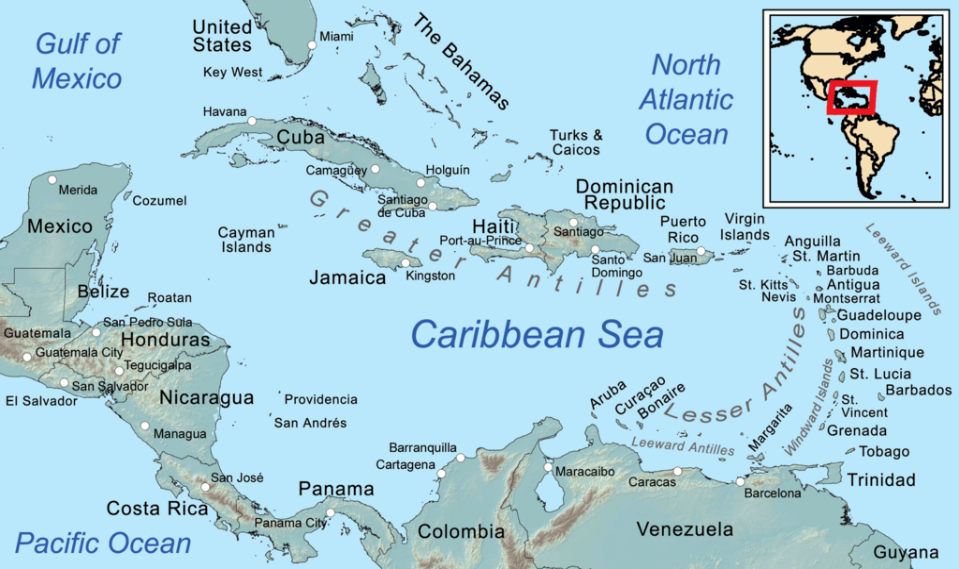
\includegraphics[width=\textwidth]{figures/delgado-img3.png}
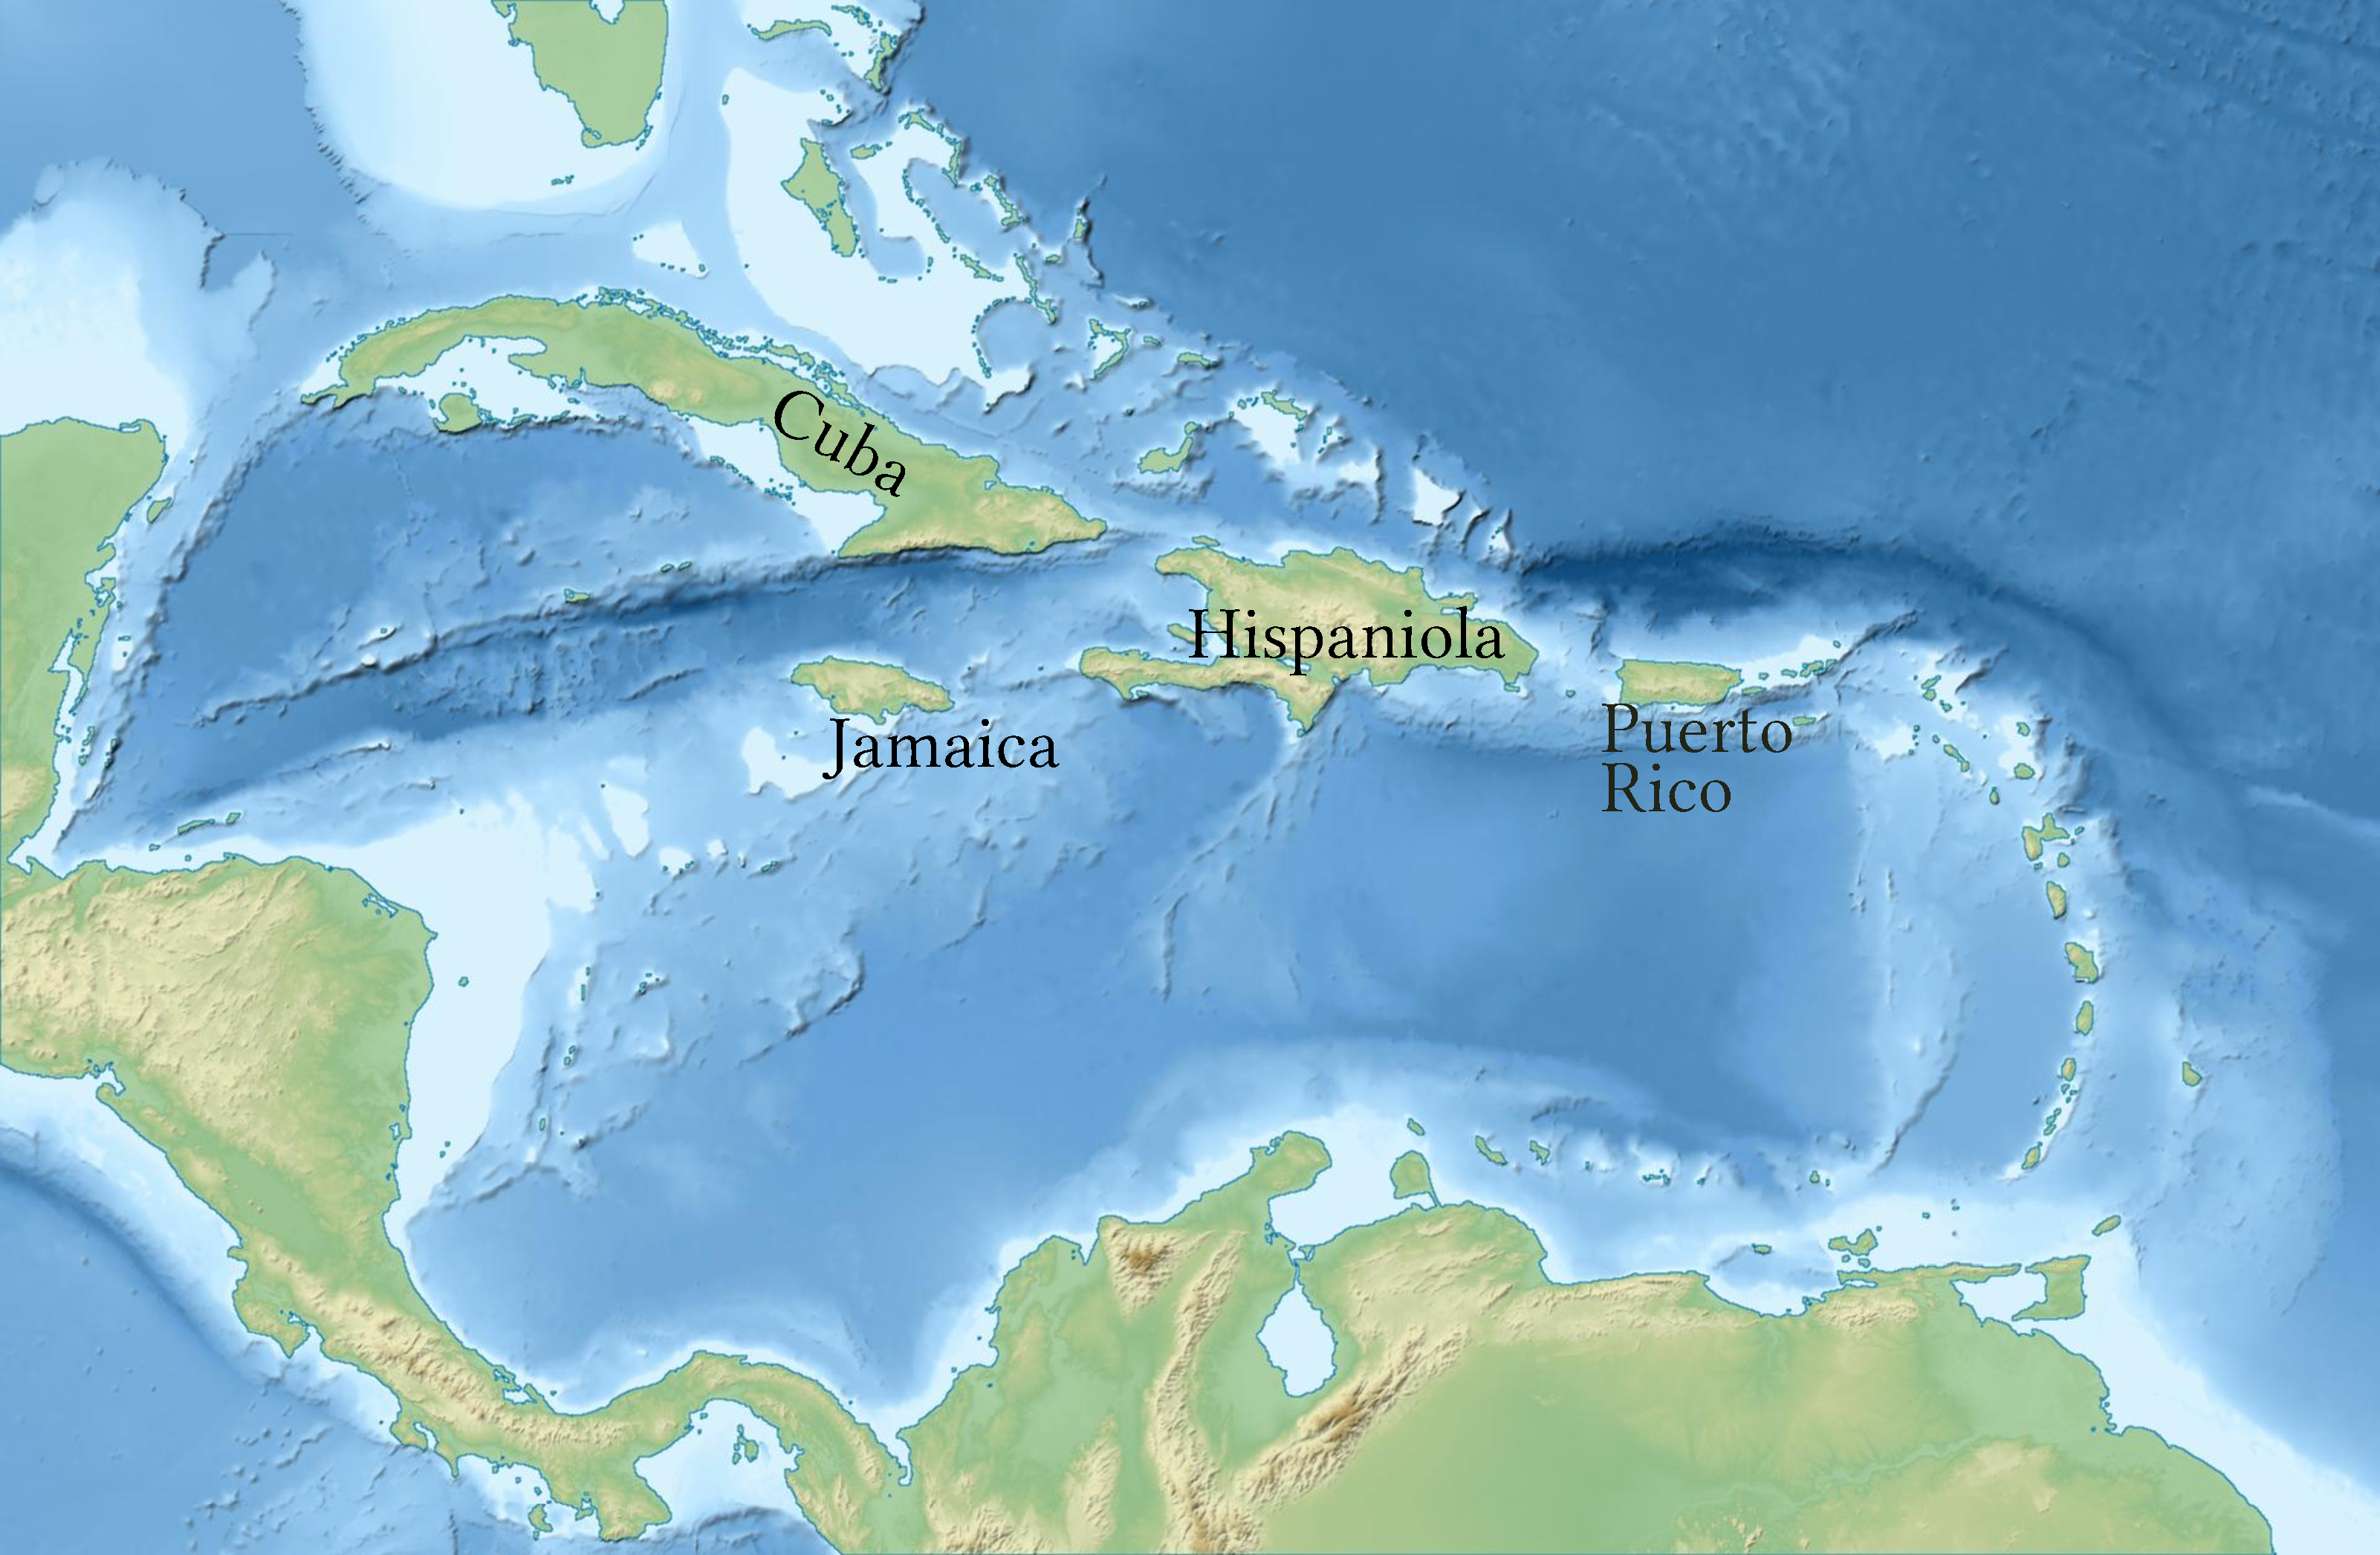
\includegraphics[width=\textwidth]{figures/img3-base.pdf}
 
\end{figure}

\begin{figure}

 

% 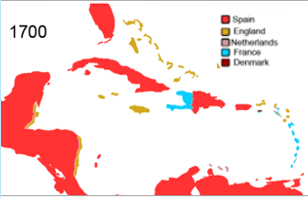
\includegraphics[width=\textwidth]{figures/delgado-img4.png}
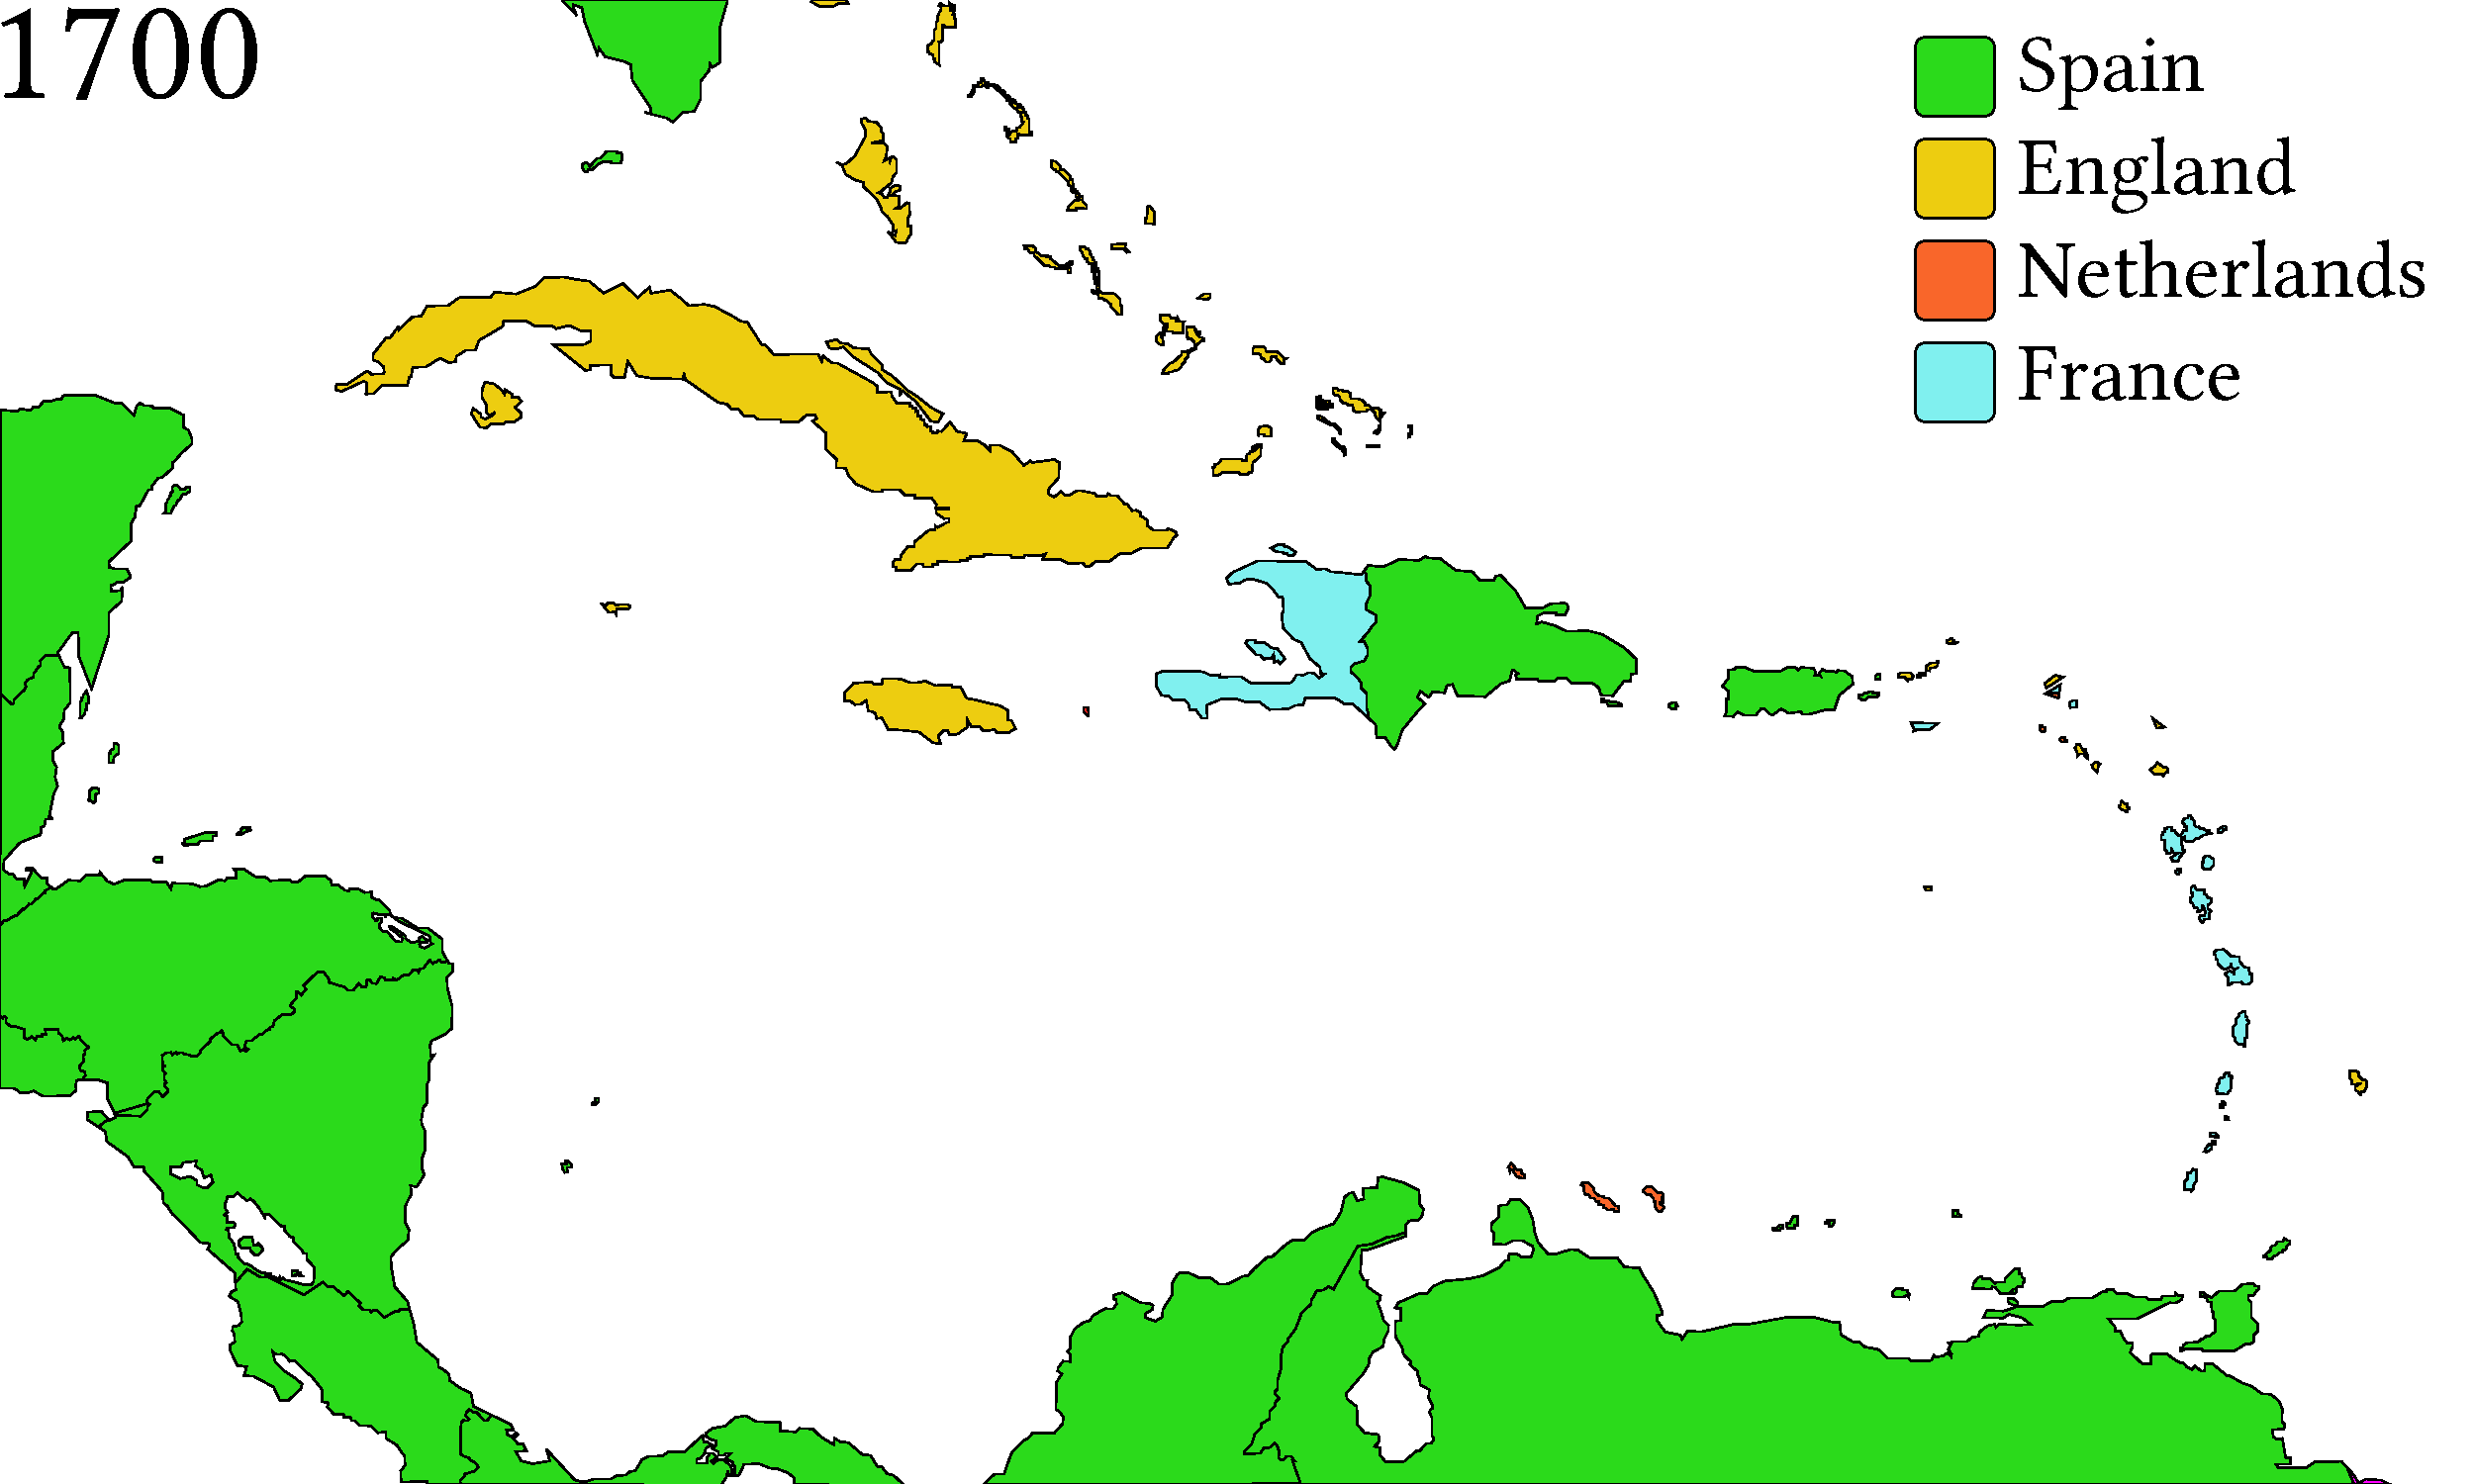
\includegraphics[width=\textwidth]{figures/img4-base.pdf}

\caption{\label{fig:key:3.4} Political Map of Central America and the Caribbean in 1700. 
% \citet{Esemono2009} “Political Evolution of Central America and the Caribbean” available in the Public Domain.
}
\end{figure}

Plurilingualism benefitted not only commanding officers who might be interested in illicit trading not sanctioned by colonial embargoes, but also individual sailors who often carried items to \isi{barter} or sell on the journey, a practice encouraged to mitigate the impact of wage arrears and promote a more incentive-based system (\citealt{Jarvis2010}: 148). Furthermore, Jarvis describes the Atlantic commons\footnote{The “Atlantic commons” refers to the public resources of the whole Atlantic region that were not explicitly owned, settled or regulated by any one nation at the time, e.g., salt deposits, shipwrecks, coastal forests, maritime trade routes, and sea-life such as whales, turtles, fish, and reefs (see \citealt{Jarvis2010}: 185–256).} as incubators of “polyglot seasonal communities, made up of English, Scottish, and Anglo-American men, Indian women, and Hispanic African runaways and slaves” (\citeyear*{Jarvis2010}: 220); Fusaro explains how difficult it is to determine the nationality of commercial shipping in the \isi{seventeenth century} given the range of national interests and \isi{crew} on board (\citeyear*{Fusaro2015}: 5); and Bicheno shows how navigational technology, shipbuilding practices, and trade routes were transferred among Spanish, Portuguese, English, Dutch and French fleets (\citeyear*{Bicheno2012}: 113). Such collaboration would have necessarily required communication and therefore some level of plurilingualism in maritime communities such as evidenced in the fact that St. Croix’s \textit{Royal Danish American Gazette} printed stories in five languages (\citealt{Jarvis2010}: 138). Evidence, albeit circumstantial, of such international collaboration abounds in the archival records, e.g., the logbook of the \textit{St. Andrew} that refers to “the signal being made foure saile of Hollanders Came into our fleet” [ADM 52/2/2]; a \isi{witness deposition} that describes “a french pinck 10 or 11 English men \& 3 french boyes on board and theire they joined forces” [HCA 1/12/4]; another testimony from a commander who explains how “two Spaniards came… he not only gave them leave so to doe but also invited them on board his sloop \& treated them very kindly” but when they robbed him, “he saw two Dutch Sails and made up to them and told them what had happened’ [HCA 1/99 \isi{Jamaica}, Aug 23 1738]; and William Wilkinson’s 1690 communication with Royal African Company that \isi{pirate} crews “passed by both French, Dutch, Brandenburgers, Interlopers, either \textit{making merry with them as their Allies}, or not daring to take notice of them as Enemies” [BL/74/816/m/11/36/2, emphasis added]. In addition to documentary circumstantial evidence, we know that certain groups were embedded in international commerce, such as the Sephardic Jews, who “traded within and across national boundaries” \citep[20]{Jarvis2010} and likely added their linguistic contribution to the plurilingual context of international commerce in the early colonial Atlantic. 

Pirate ships were more likely than others to generate plurilingual environments and also enabled sailors with ample time to converse to acquire new languages. Indeed, plurilingualism became, at the time, a marker of guilt and complicity in piratical activity, as illustrated by J. Moreland’s testimony, “must I be hanged that I can speake all languages” [CO 5/1411/56] and the accusation that one \isi{prisoner} heard his captors “profanely Singing at suppertime Spanish and French Songs out of a Dutch Prayer Book” [HCA 1/99/139]. Atlantic historians Linebaugh and Rediker describe the \isi{pirate ship} as “motley — multinational, multicultural, and multiracial” (\citeyear*{LinebaughRediker2000}: 164) and colonial historian McDonald, explains how “pirates served as important cross-cultural brokers in the early modern world” facilitating collaborative efforts among logwood cutters and local indigenous populations in colonial America (\citeyear*{McDonald2016}: 1).  Pirate crews also notoriously rejected national allegiance, described by one administrator, “they are governed by no laws of nation” [CO 5/1411/44], an attitude corroborated by the logbook of the \textit{\isi{Essex} Prize} in the 29 August entry for 1698 which describes how “they [the \isi{crew} of the \textit{\isi{Essex} Prize}] could not liarn by any means which way he was bound or from whence he [the \isi{pirate ship}] came for they all told you they were bound to sea” [CO 5/1411/691]. This rejection of national allegiance, demonstrated visibly with the black ensign, was also likely demonstrated linguistically with the rejection of European standard forms of speech (\citealt{Delgado2013}: 157–158). This rejection potentially took the form of \isi{new dialect} genesis, code-switching, and the rejection of a single lingua franca, characteristics that pirates potentially transferred to their freebooting havens in places like Port Royal, \isi{Jamaica}; Ile Sainte-Marie, Madagascar; Tortuga, Haiti; and the Isle of Wight, England, described as “a hub for corsairs of all nations” (\citealt{Bicheno2012}: 41). 

Among the profusion of circumstantial evidence that sailors were plurilingual, occasional direct evidence also attests to sailors’ language abilities. In a rare statement about linguistic abilities in court documents, a description of Charles Macarly states, “the examinant speaks English Irish and a Little Flemmish” [HCA 1/13/96]. Also, Earle’s extensive work on the demographics of English  Sailors 1570–1775 cites evidence of Nicholas Lawrence who, despite being illiterate, “has been so much abroad as to be able to speak French, Spanish, Italian, Portuguese” and his shipmate Peter Breton could “speake French and English and a little of the Lingua Franca” (\citeyear*{Earle1998}: 21). Earle also cites information on the Bicknell brothers, who served on the privateer \textit{Swallow} and both spoke Latin, French, Dutch, and “a little broken Spanish and Portuguez” (\citeyear*{Earle1998}: 21). One \isi{sailor} working at the end of the \isi{eighteenth century} describes the plurilingual tradition of the seas in his astonished reaction to naval recruitment aboard British naval vessels, “to the ear was addressed a hubbub little short of that which occurred at Babel. Irish, Welsh, Dutch, Portuguese, Spanish, French, Swedish, Italian and all the provincial dialects between Landsend and John O’Groats” (cited in \citealt{AdkinsAdkins2008}: 11). Thus, contemporary accounts indicate that not only English dialects from around the British Isles were likely to have been present aboard ships, but also a range of languages, most notably from seafaring European powers yet also potentially from regions of the littoral Atlantic. 

Evidence of French, Spanish, Portuguese, Dutch, Italian, and also unspecified African languages are attested to in depositions, letters and logbooks, in addition to Latin that most upper-class people would have been exposed to through formal education. Perhaps not surprisingly, given the geographical proximity of France and Spain and also the importance of these countries in the definition of the religious and political ideology of Britain at the time, French is the language most frequently named in accounts of on-board bilingualism, followed by Spanish. Indeed, speaking French had been a maritime tradition reinforced in the \isi{sixteenth century} as French corsairs inspired the first waves of Elizabeth I’s privateering ventures led by \isi{Drake}, who “became the heir of the French corsair tradition [and] [...] must have spoken French fluently” (\citealt{Bicheno2012}: 113). Moreover, as Adkins and Adkins note, up until the \isi{eighteenth century}, “French was not only the language of England’s principal enemy, but the language of trade and politics in many parts of the world” (\citeyear*{AdkinsAdkins2008}: 22). Certain accounts indicate that it was the commanding officers who spoke French, e.g., one passenger account dated 1666 describes the captain’s language abilities, “he spoke to them in French, because they had put up white colours” [445f.1/511] and Captain Vaughan engages one man who “can speak nothing but French” and another who “speaks Walloon \& French and no other language” [HCA 1/13/95]. The officers’ language abilities, most probably a result of formal schooling, was then potentially extended by contact with other languages in the rich environment of the plurilingual seas. For instance, one ship’s clerk is described in court documents thus, “he speaks French and Latin and some few words in Dutch but cannot speak yet any other language” [HCA 1/13/96]. The clerk most likely learned French and Latin through formal schooling, but the fact that he spoke basic Dutch seems to imply a more recent acquisition, Also, the use of the words “cannot speak \textit{yet} any other language” (emphasis added) implies that the court officials anticipate further \isi{language acquisition} as a result of his presence on the ship. Most able seamen, unlikely to have gone through formal education, may have also acquired languages by contact, e.g. the 1696 witness testimony of 46-year-old John Morphey who “hath sailed to and from severall places by the West Indies… and the reason why he can now speak a little French is because he sailed for the most part amongst other sailors [...] onboard a french privateer” [HCA 1/53/9]. Such \isi{language acquisition} may have been a natural process for many sailors who were in frequent contact with foreigners, as illustrated (albeit on a much smaller scale) by a journal of one passenger who notes how African natives of the coast “were to carry us to one of their towns, which in their language they call \textit{libattes}, as we shall always call them in this relation” [445f.1/492].  So, even in this much more restricted context of linguistic borrowing, there is nonetheless an indicator that wider \isi{language transfer} was happening that was potentially ubiquitous among multinational crews. 

The extent of foreign colonies in the New World and the consequent emergence of a plurilingual \isi{transatlantic} trade meant that language abilities were pivotal skills for many mariners of the age, as shown by the \isi{crew} of the English \textit{St. Peter}, who are described as “speaking Spanish \& after that Dutch to them in the Canoa” [HCA 1/9/14]. And on a wider scale, the \isi{merchant} fleets of an entire nation were served by the language abilities of their enlisted \isi{crew}. Fusaro’s research into seventeenth-century Venetian court records “provides a powerful impression of the international composition the crews of the ships involved” (\citeyear*{Fusaro2015}: 16). She concludes that foreign seafarers in Venetian fleets, many of whom were English, had considerable linguistic knowledge based on the fact that only in rare cases did any of them need interpreters in Italian courts (\citealt{Fusaro2015}: 17). Contemporary allusions to interpreters also attest to the value of language abilities in contexts of trade, e.g., John Everett, deposed in court 1700, is described as “having been then shipped [from Curaçao] [...] to go with him as Pilot and Linguister in the sloop… to trade amongst the Spanish” [SP 42/6/53]; Diego Hossa, a native of \isi{Bahama} Island, described as a “negro belonging to capt Higgingbotham” is later referred to as “a linguist or Spanish interpreter” [HCA 1/99 \isi{Bahama} Islands 1722] and, in a Letter dated 11 January {1697} addressed to Capt Cornelis Jacobs or Capt Samuele Burges, “a mollatto”, presumed to have travelled with privateer crews, is described as a person who “Speacks verry good English \& Dutch” [HCA 1/98/75]. Moreover, in the absence of an interpreter, some crews sought to train one, such as the \isi{crew} of one Portuguese vessel described in Arents’ journal, who:

\begin{quotation}
finding it impossible for them to discover any thing more, because they understood not one another, resolv’d to set sail with the first wind [...] they thought good to bring two of them along in the Vessel; in hopes that they might learn the Portuguese language, or that there might some child be found out that might understand what they said. [Arents/361 \textit{The Six Voyages} 1678: 84]\end{quotation}

  On the other hand, for English crews, trade with foreign nations was either heavily regulated or entirely banned and so knowledge that a \isi{sailor} could speak foreign languages could potentially be used as evidence for their prosecution, e.g., in one court hearing, testimony is given against the five British men accused of \isi{contraband} trade, “this said vessel commanded by Solomon Middleton who hailing you in Spanish and some of you making answer Espaniols” [HCA 1/99 \isi{Bahama} Islands 1722]. African language skills were also viewed with suspicion, e.g., in the case of William Child accused of inciting a negro revolt on board because he “had been talking to the Negroes in Angolan Language all Night” [HCA 1/99/82, 28 March {1722}]. A map of Africa by Aaron Arrowsmith submitted as part of a manuscript sent to the “British Association” in 1802 (\figref{fig:key:3.5}) although it dramatically illustrates the lack of knowledge of any territory beyond the coastal and river-basin areas of the African Continent, might provide some evidence of areas that experienced greater \isi{language contact} with Atlantic maritime communities. 

\begin{figure}
 

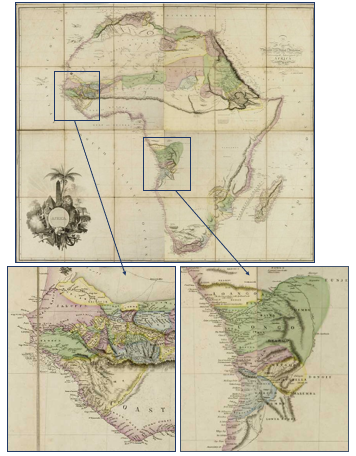
\includegraphics[width=\textwidth]{figures/delgado-img5.png}

\caption{\label{fig:key:3.5} Historical Map of Africa from a manuscript sent in 1802 written by Aaron Arrowsmith (with added regional inserts). Courtesy of the National Maritime Museum, Greenwich, London, Creative Commons license CC-BY-NC-SA-3.0}
\end{figure}

The two areas on the Atlantic coast for which more details are provided (both expanded) correspond roughly to the far west coastal areas of modern-day Senegal, the Gambia, Guinea-Bissau, Guinea and Sierra Leone and the more southerly Angola. This may suggest that the Niger-Congo language family was more heavily represented in Atlantic maritime communities during the period under study, specifically Fula and Mande languages on the far west coastal regions and Bantu languages of modern-day Angola, and potentially also Kru, Kwa/Igbo and other Volta-Niger languages of the West African coast that connected the two regions. The details provided for South Africa and Pacific regions (modern-day Mozambique and Madagascar) may suggest that Khoisan was present but certainly implies that pacific varieties of languages of the Bantu family entered the \isi{maritime language} contact situation (\figref{fig:key:3.6}). In sum, English-speaking sailors often had foreign language abilities that would have been considered unusual for those in professions on land, whether that meant extensive single-word borrowing, a basic competency for trade, or near-native fluency. 

  
\begin{figure}

% 
\includegraphics[width=\textwidth]{figures/delgado-img6.png}

\includegraphics[width=\textwidth]{figures/img6-base.pdf}
 
\caption{\label{fig:key:3.6} Map of the Atlantic-Congo languages within the Niger-Congo language family. {\tiny © Eric Gaba CC BY-SA 4.0}} 
\end{figure}

\section{{Literacy}}\label{sec:3.11}

  Despite their spoken competency, most sailors were not proficient in reading or writing in any language. Linguistic skill but poor literacy is illustrated in one deposition of a \isi{sailor}, “sent to sea at a very tender age as cabin-boy and had no education [...] he could never read a word in a book…[but] he has been so much abroad as to be able to speak French, Spanish, Italian, Portuguese” (cited in \citealt{Earle1998}: 21). Indeed, most working class people in Britain were illiterate before the Elementary Education Act of 1870 made schooling compulsory, and common seamen were no exception to this general trend (\citealt{AdkinsAdkins2008}: 345). One rare court record of the testimony of John Morphey in 1696 includes an explanation “that he was examined at Plymoth and that he cannot write” [HCA 1/53/9], and in a context when the illiteracy of sailors would have been assumed, this may only be provided to explain why the \isi{deponent} did not put his mark on the document. Some type of personal mark would have been a routine procedure for enlistment and was also expected in court documentation to corroborate a testimony written by a \isi{court clerk}. Pervasive examples of such personal marks in the court documentation include the shaky crosses penned by anonymous seamen unaccustomed to holding pens, legible initials, and also full names signed with a flourish (see \figref{fig:key:3.7}). Yet, even in consideration of Earle’s claims that “some two-thirds of ordinary foremastmen and over 90 percent of men who held any type of office in a ship could sign their names” \citep[20],{Earle1998} the large quantity of testimonies marked with the letter <x> or initials compared to those signed with a legible name support the previous claim that the majority of sailors were functionally illiterate. 

\begin{figure}
  

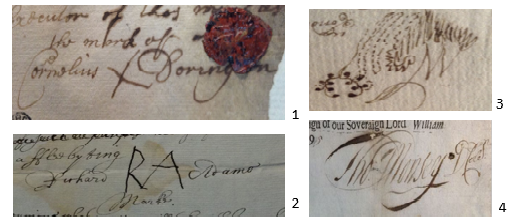
\includegraphics[width=\textwidth]{figures/delgado-img7.png}
 

\caption{\label{fig:key:3.7} Examples of personal marks corroborating testimony in seventeenth century depositions and documents prepared by or on behalf of sailors, sources: 1. HCA 1/98/85; 2. HCA 1/101/220; 3. HCA 1/98/173; 4. HCA 1/98/62}
\end{figure}

Certain sailors who would have been expected to have some degree of literacy are, for instance, all commanding officers, the master, boatswain, purser, carpenter, shipwright, and boys first class. The duties of such positions would have required functional literacy, e.g., the shipwright’s assistant who needed to prepare a certificate relating to the condition of the timber for Commander Beach [ADM 106/288/35]. Earle further explains, “a boatswain [...] had to be able to check manifests, read bills of lading and give receipts for merchants’ goods delivered aboard” (\citeyear*{Earle1998}: 21) and sailors could be disciplined or lose their position if unable to complete the tasks of their rank, e.g., the Boatswain of the \textit{Elizabeth} who was dismissed because he “write very indifferently, very slow, could not spell” (cited in \citealt{Earle1998}: 21). Carpenters were required to be literate, but more importantly to perform extensive calculations, as were ships’ officers in charge of determining nautical speed, distance covered and latitude. Thus, numeracy determined competency for many sailors more so than literacy and this is reflected in the educational provisions for wealthy families’ children during the \isi{seventeenth century}. Young boys on the threshold of service at sea were commonly removed from grammar school and placed in specialized occupational schools that were often run by accountants or retired seamen, bypassing the more traditional curriculum in Latin, rhetoric and grammar.  Instead these boys were trained in the more practical skills of record keeping, mathematics and navigation (\citealt{Earle1998}: 22). 

Indeed, such skills were paramount if the recruit had ambitions for a naval career and, as a result, numeracy and literacy rates were high among officers. Nonetheless, even literate officers were less exposed to texts and had fewer demands on them to read or write in comparison with standards of today.\footnote{A comparison with the compulsory education of a wealthy nation in the twenty-first century is intended, with full acknowledgement of varying global standards of literacy and compulsory schooling.} To illustrate, in the 1700 trial of a Newfoundland chief officer of forces [SP 42/6] various ship masters were alleged to have read and signed a fraudulent certificate, yet, in their defense, Captain Fairbourne explains that “most of them declared that mr. B. handed the certificate to them, and that they were ignorant of the full contents thereof” seeming to suggest that their literacy was not equal to the comprehension of the full document. In another case, a literate \isi{sailor} who witnessed the crime being tried in a court case in 1731 sent a letter to the court to serve as his testimony, yet this same letter is described as being “conceived in Terms not very intelligible” and therefore the author is sent for “to explain the meaning” [HCA 1/99/9]. Miscomprehension may have been perpetuated by idiomatic language usage, local \isi{dialect} and non-standardized spelling,\footnote{Variation in spelling would have been the norm during the early \isi{colonial period} in question (1620–1750) before standardization of prestigious dialects were codified in prescriptive grammars of the \isi{eighteenth century} and disseminated in the compulsory education of the nineteenth century.} but both these examples suggest that sailors considered literate by virtue of their abilities to read and write may not have been able to read or write across a wide range of dialects, registers or styles as we might determine full literacy today.  

  In lieu of formal schooling, a common \isi{seaman} may have learned basic literacy the same way that they learned languages, i.e., among crewmates in leisure hours. Jarvis supports this supposition by observing that “seafaring both facilitated and promoted reading: circumatlantic passages provided sailors with ample reading time, and their visits to major seaports helped them procure books” \citep[307],{Jarvis2010} a claim which supports Earle’s observation that “schooling was important, but a \isi{sailor}’s real education began at sea” (\citeyear*{Earle1998}: 22). Certainly, a small number of functionally literate lower-ranking sailors were likely to have been in great demand when it came to reading and responding to letters from home, and some sailors, no doubt, pressed these scribes to learn how to communicate with loved ones in their own hand. Some personal letters, or copies of such letters, written by common sailors survive in the Admiralty’s court papers, e.g., one letter produced as evidence against John Seaman and described “with the hand writing of the defendant [...] beginning with those words Deare father and ending with those words your obedient sone [...] Seaman” [C 22/710/50] and four letters brought as evidence against Alexander Wyatt “who owned them to be in his own Hand Writing” [HCA 1/99 \isi{Bahama} Islands 1722]. Other evidence survives in miscellaneous documentation, e.g., a series of short letters regarding the will of John Read in relation to his wife [HCA 1/98/92–96] and a personal letter dated April 13 1699 from “Abraham [surname unintelligible] [...] serving aboard Captain Kidd’s vessel to his wife Margaret expressing “my Love to you and to our Child” [HCA 1/98/172]. The fact that some letters from literate wives also survive in the records speaks to the anticipated literacy of crewmen, e.g. one wife who writes simply to her “Deare And Loving husband” [HCA 1/98/116] and another who gives evidence of a continued communication in her comment “I have sent you two letters before this and have Received One” [HCA 1/98/118]. Some surviving seamen’s journals also contain samples of writing, e.g., the images and notes in Basil Ringrose’s journal, dated 1682 [The National Maritime Museum, exhibit P/32] and the comments on Charles II’s return from exile in 1660 in Edward Barlow’s journal, in which the surprisingly literate \isi{seaman} describes how people saluted the returning king “as though they were all glad to bear him up and have the happiness to welcome home the true sovereign [...] for whom the land had so long grieved” [The National Maritime Museum, exhibit JOD/4f.24]. In conclusion, although numerous indicators suggest that the majority of common seamen were illiterate, rates of literacy among officer ranks were high and there is also evidence that some common sailors were literate, potentially for the purposes of their jobs, and these likely served as readers, writers, and teachers to illiterate crewmates. 

\section{{Number of sailors on the ships}}\label{sec:3.12}

  Determining the likely number of sailors on ships during the early \isi{colonial period} in the Atlantic and Caribbean is feasible, but only through analysis of incomplete and fragmentary data. Muster rolls detailing \isi{crew} lists for British naval vessels did not appear until the mid-\isi{eighteenth century} \citep[125]{Litter1999} and the Lloyd’s registers of vessels that may have also detailed \isi{crew} numbers was not established until about the same time (\citealt{Litter1999}: 191). However, individual ships kept records on their crews, some of which survive in Admiralty archives, and from such miscellaneous records it is possible to make valid assertions about population demographics aboard individual vessels. Based on 22 vessels for which I found first-hand accounts (in the same document) of both the ship size and the size of the \isi{crew} for Atlantic or Caribbean voyages, there was an average of 115 men in a 21-gun 239-ton vessel, or to express the data in terms more suited to the contemporary manning requirements, the equivalent of 6.39 guns per man or 2.35 tons per man (see \tabref{tab:key:3.4}). These figures are comparable to the late-\isi{sixteenth century} optimum of one man per two tons of ship’s weight for long voyages (Hawkins, cited in \citealt{Bicheno2012}: 127), the only changes being that in the seventeenth and eighteenth centuries, larger ships were built with more guns and therefore larger crews were needed to equip them, culminating in the 100-gun warship of Nelson’s navy enlisting an average of 837 men (The National Maritime Museum, “Nelson Navy Nation” exhibition).

\begin{table}
\caption{\label{tab:key:3.4} Number of crew in transatlantic and Caribbean vessels based on first-hand accounts in the National Archives and Merseyside Maritime Museum holdings}
\footnotesize
\begin{tabularx}{\textwidth}{lrYYYYl}
\lsptoprule

& \textbf{Guns} &  \textbf{Tons}\textsuperscript{a} &  \textbf{Men} & \textbf{Guns/Man} & \textbf{Tons/Man} & \textbf{Source document}\\
 \midrule
& 44 &  499 &  84 & 1.9 & 5.9 & HCA 1/53/13\\
& 40 &  454 &  80 & 2.0 & 5.7 & HCA 1/53/12\\
& 18 &  204 &  65 & 3.6 & 3.1 & HCA 1/98/9 \\
& 18 &  204 &  65 & 3.6 & 3.1 & HCA 1/98/258\\
& 40 &  454 &  150 & 3.7 & 3.0 & HCA 1/98/265\\
& 22 &  249 &  90 & 4.0 & 2.8 & HCA 1/98/3\\
& 22 &  249 &  90 & 4.0 & 2.8 & HCA 1/98/263\\
& 12 &  136 &  50 & 4.1 & 2.7 & 1045.f.3/1/15\\
& 26 &  295 &  130 & 5.0 & 2.3 & CO 5/1411/631\\
& 26 &  295 &  130 & 5.0 & 2.3 & CO 5/1411/690\\
& 16 &  181 &  80 & 5.0 & 2.3 & CO 5/1411/99\\
& 12 &  136 &  70 & 5.8 & 1.9 & CO 5/1411/636\\
& 18 &  204 &  110 & 6.1 & 1.8 & HCA 1/98/11\\
& 18 &  200\textsuperscript{b} &  110 & 6.1 & 1.8 & HCA 1/98/262\\
& 8 &  90 &  50 & 6.2 & 1.8 & CO 5/1411/691\\
& 14 &  158 &  88 & 6.2 & 1.8 & HCA 1/99/9\\
& 4 &  45 &  30 & 7.5 & 1.5 & CO 5/1411/636\\
& 70 &  794 &  650 & 9.2 & 1.2 & HCA 1/53/18\\
& 10 &  150\textsuperscript{b} &  110 & 11 & 1.4 & HCA 1/52/94\\
& 10 &  113 &  120 & 12 & 0.9 & HCA 1/98/7\\
& 10 &  113 &  120 & 12 & 0.9 & HCA 1/98/256\\
& 4 &  45 &  66 & 16.5 & 0.7 & HCA 1/52/176\\
 \midrule 
Average &  \textbf{21} &  \textbf{239} &  \textbf{115} & \textbf{6.39} & \textbf{2.35} & \\
\lspbottomrule
\end{tabularx}
\parbox{.95\textwidth}{\footnotesize
\textsuperscript{a}Conversions based on an estimated 11.35 tons/gun derived from 58 warships for which we have tonnage and gun capacity (\citealt{Bicheno2012}: 353, 358–361). \\
\textsuperscript{b}Tonnage given in archival record (not estimated)
}
\end{table}

Large crews were a feature of ships which had a high \isi{crew} turnover due to death, injury, disciplinary measures and desertion, and because of this, “overcrowding generated the diseases that were the greatest danger on long voyages” (\citealt{Bicheno2012}: 78). Additionally, in periods of heightened conflict, overmanning ships became a necessary procedure in the anticipation of seizing vessels and equipping them with a functional \isi{crew}. This tendency to recruit large crews was consequently exaggerated in \isi{pirate} crews, as suggested by one witness testimony of 28 March {1722}, in which one \isi{deponent} describes “a Boat which they Supposed \textit{by the number of Men in her} were Pirates” [HCA 1/99/24, emphasis added]. Furthermore, warships operating in the \isi{transatlantic} waters had significantly increased \isi{crew} for the requirements of navigation and defense. Such large ships weighing between 220 and 760 tons operated with an average \isi{crew} of 278 (including troops) based on 28 late sixteenth-century English warships for which we have this data (\citealt{Bicheno2012}: 355). However, extensive variation among vessels would have been determined by the size of the vessel, the type of \isi{voyage}, the preferences of the captain, recruitment procedures, availability of workers, the anticipated \isi{crew} depreciation, cargo requirements, and the age, defense system and navigational rigging of the vessel. Small crews served the short-range trading vessels of the wider Caribbean, for instance, “four to eight men were generally sufficient to man a [Bermuda] sloop” \citep[123]{Jarvis2010} and only ten men were needed to man the 20-ton 3-gun Pinnace \textit{Black Dog} listed for Royal hire and registered in London (\citealt{Bicheno2012}: 352). Comparatively, the largest crews of the warships could exceed 500 enlisted men, e.g., the 340 \isi{crew} and 160 troops (500 total) aboard the 760-ton 42-gun Royal Carrack \textit{Triumph} \citep[355],{Bicheno2012} the evidence of one testimony of a ship of “70 gunns and abt 600 or 700 men” [HCA 1/53/18], and the note in the Boatswain’s log of the \textit{St Andrew} to have “hammocks delivered to the men [...] five hundred” [ADM 52/2/3]. However, even given these large \isi{crew} numbers, the estimated numbers of people aboard any vessel are likely to be extremely conservative in light of the assumption that slaves, servants, women, and non-enlisted children were not counted as they entered the ships through means other than official enlistment and did not appear on wage registers or \isi{crew} manifests. 

\section{{Summary}}\label{sec:3.13}

  This chapter re-defines the word “\isi{sailor}” to refer to all sea-going workers of the early \isi{colonial period} under study and presents sections on demographics with full acknowledgement of the limitations and complexities of data collection and analysis. Recruitment of sailors included voluntary enrollment; conscription; and the assignment of impressed, indentured, enslaved, and detained populations. Most sailors in lower ranks would have been enlisted via methods involving some degree of coercion, manipulation, or outright force and were routinely kept at sea for long periods without shore leave for fear of desertion. Although popular stereotype assumes that all sailors were male, a minority of women worked on ships as \isi{crew}, collaborators, and service providers. Most sailors were young, going to sea in their early teens and serving typically until the age of around fifty with an average \isi{crew} age of around thirty. Poor hygiene, putrid food, overcrowding, and lack of clean water, as well as hard labor, exposure to environmental risks, and wounds caused by disciplinary action or military conflict, resulted in high sickness and mortality rates. Sailors had strong family ties and many served alongside fathers, uncles and sons at sea. Furthermore, and contrary to popular stereotypes, sailors commonly married and had children, and their wives were active in maritime communities, sometimes accompanying their husbands to sea. Ranks determined social status at sea and composed a rigid hierarchy: the privileged upper class, the trade and military middle class, and the seamen of the largest lower class, potentially supplemented by a sub-category of undocumented, unpaid, or forced workers. Theoretically, wages were paid and could be supplemented by various means, but in reality, sailors’ wages were perpetually in arrears and paid intermittently and insufficiently if at all, a situation that commonly led to conflict, \isi{mutiny}, and thus potential imprisonment and death. Most sailors born in the geographical British Isles were English, followed by the Irish, Scots and Welsh.  London{}-born sailors were most heavily represented in naval vessels, coastal northerners in the \isi{merchant service} and coastal southerners and westerners in privateering and piracy. The Commonwealth’s extended interpretation of what it meant to be British meant that sailors were often recruited from British territories, including the Caribbean and the 13 colonies of North America but were also heavily recruited from the sea-going nations of Europe. English was the default language aboard British ships and so some sailors may have been monolingual. However, more commonly, English-speaking sailors had foreign language abilities that were acquired directly from \isi{language contact} in their maritime communities and were essential in the context of the \isi{transatlantic} trade. On the other hand, plurilingualism may have been an occupational hazard as it exposed common sailors to capture for the purposes of interpreting and also suggested they were guilty of piracy considering that \isi{language contact} and therefore \isi{language acquisition} was perceived as more profuse aboard such vessels. The majority of sailors were illiterate; yet certain positions would have required some degree of functional literacy. Moreover, officers were likely to have had comparatively high levels of literacy and numeracy, and some common seamen may have learned basic literacy among crewmates in leisure hours for purposes of personal communication. Relating to numbers of men on the ships, there was a conservative average of 115 men in a 21-gun 239-ton vessel comparable to the \isi{sixteenth century} optimum of one man per two tons of ship’s weight for long voyages. However, \isi{crew} sizes were increasing throughout the period under study due to the use of larger ships and piracy. 

